% \chapter{Implementación} \label{implementacion}

% En este capítulo, se va a describir detalladamente la implementación de este proyecto. Primeramente, definiremos el entorno de desarrollo para más adelante poder abordar la implementación de la API, la implementación del acceso a la base de datos, la implementación de funcionalidades avanzadas de Spring Boot, la implementación del login, la implementación de la vista con Thymeleaf y, por último, las funcionalidades extras que hacen del proyecto una aplicación altamente versátil.

% \section{Entorno de desarrollo}

% El entorno de desarrollo utilizado para este proyecto se basa en un equipo portátil con las siguientes características técnicas:

% \begin{itemize}
%     \item Sistema operativo: Windows 11.
%     \item Memoria \acrshort{ram}: 16 \acrshort{gb}.
%     \item Procesador: Intel Core i7.
% \end{itemize}


% Esta configuración ha permitido un rendimiento fluido durante las distintas etapas del desarrollo, desde la programación hasta las pruebas de la aplicación, por lo que el uso de un dispositivo de características similares para recrear el proyecto sería más que suficiente.

% Para la implementación del sistema, se ha utilizado el entorno de desarrollo integrado (o \acrshort{ide}) Eclipse, versión 4.28.0. Eclipse es ampliamente reconocido por su soporte robusto para proyectos Java y su integración con herramientas como Maven, facilitando la gestión de dependencias y el ciclo de vida del proyecto, como se ha explicado anteriormente.

% El proyecto se ha desarrollado utilizando el marco de trabajo Java Spring Boot en su versión 2.7.18. Recordemos que Spring Boot es una herramienta poderosa para la creación de aplicaciones Java empresariales, ya que simplifica la configuración inicial y proporciona una estructura robusta para aplicaciones web.

% El lenguaje de programación empleado ha sido Java, utilizando el \acrfull{jdk} 1.8. Este entorno de ejecución permite una amplia compatibilidad con bibliotecas y herramientas esenciales para el desarrollo.

% Para la gestión de dependencias, compilación y empaquetado del proyecto, se ha utilizado Apache Maven en su versión 4.0.0. Maven permite gestionar las bibliotecas externas de manera eficiente, garantizando que todas las dependencias estén sincronizadas y disponibles en las versiones correctas. Esto se configura a través del archivo `pom.xml`, que define las dependencias necesarias y sus versiones, como se puede ver en la Figura \ref{fig:maven_pom}.

% \begin{figure}
%     \centering
%     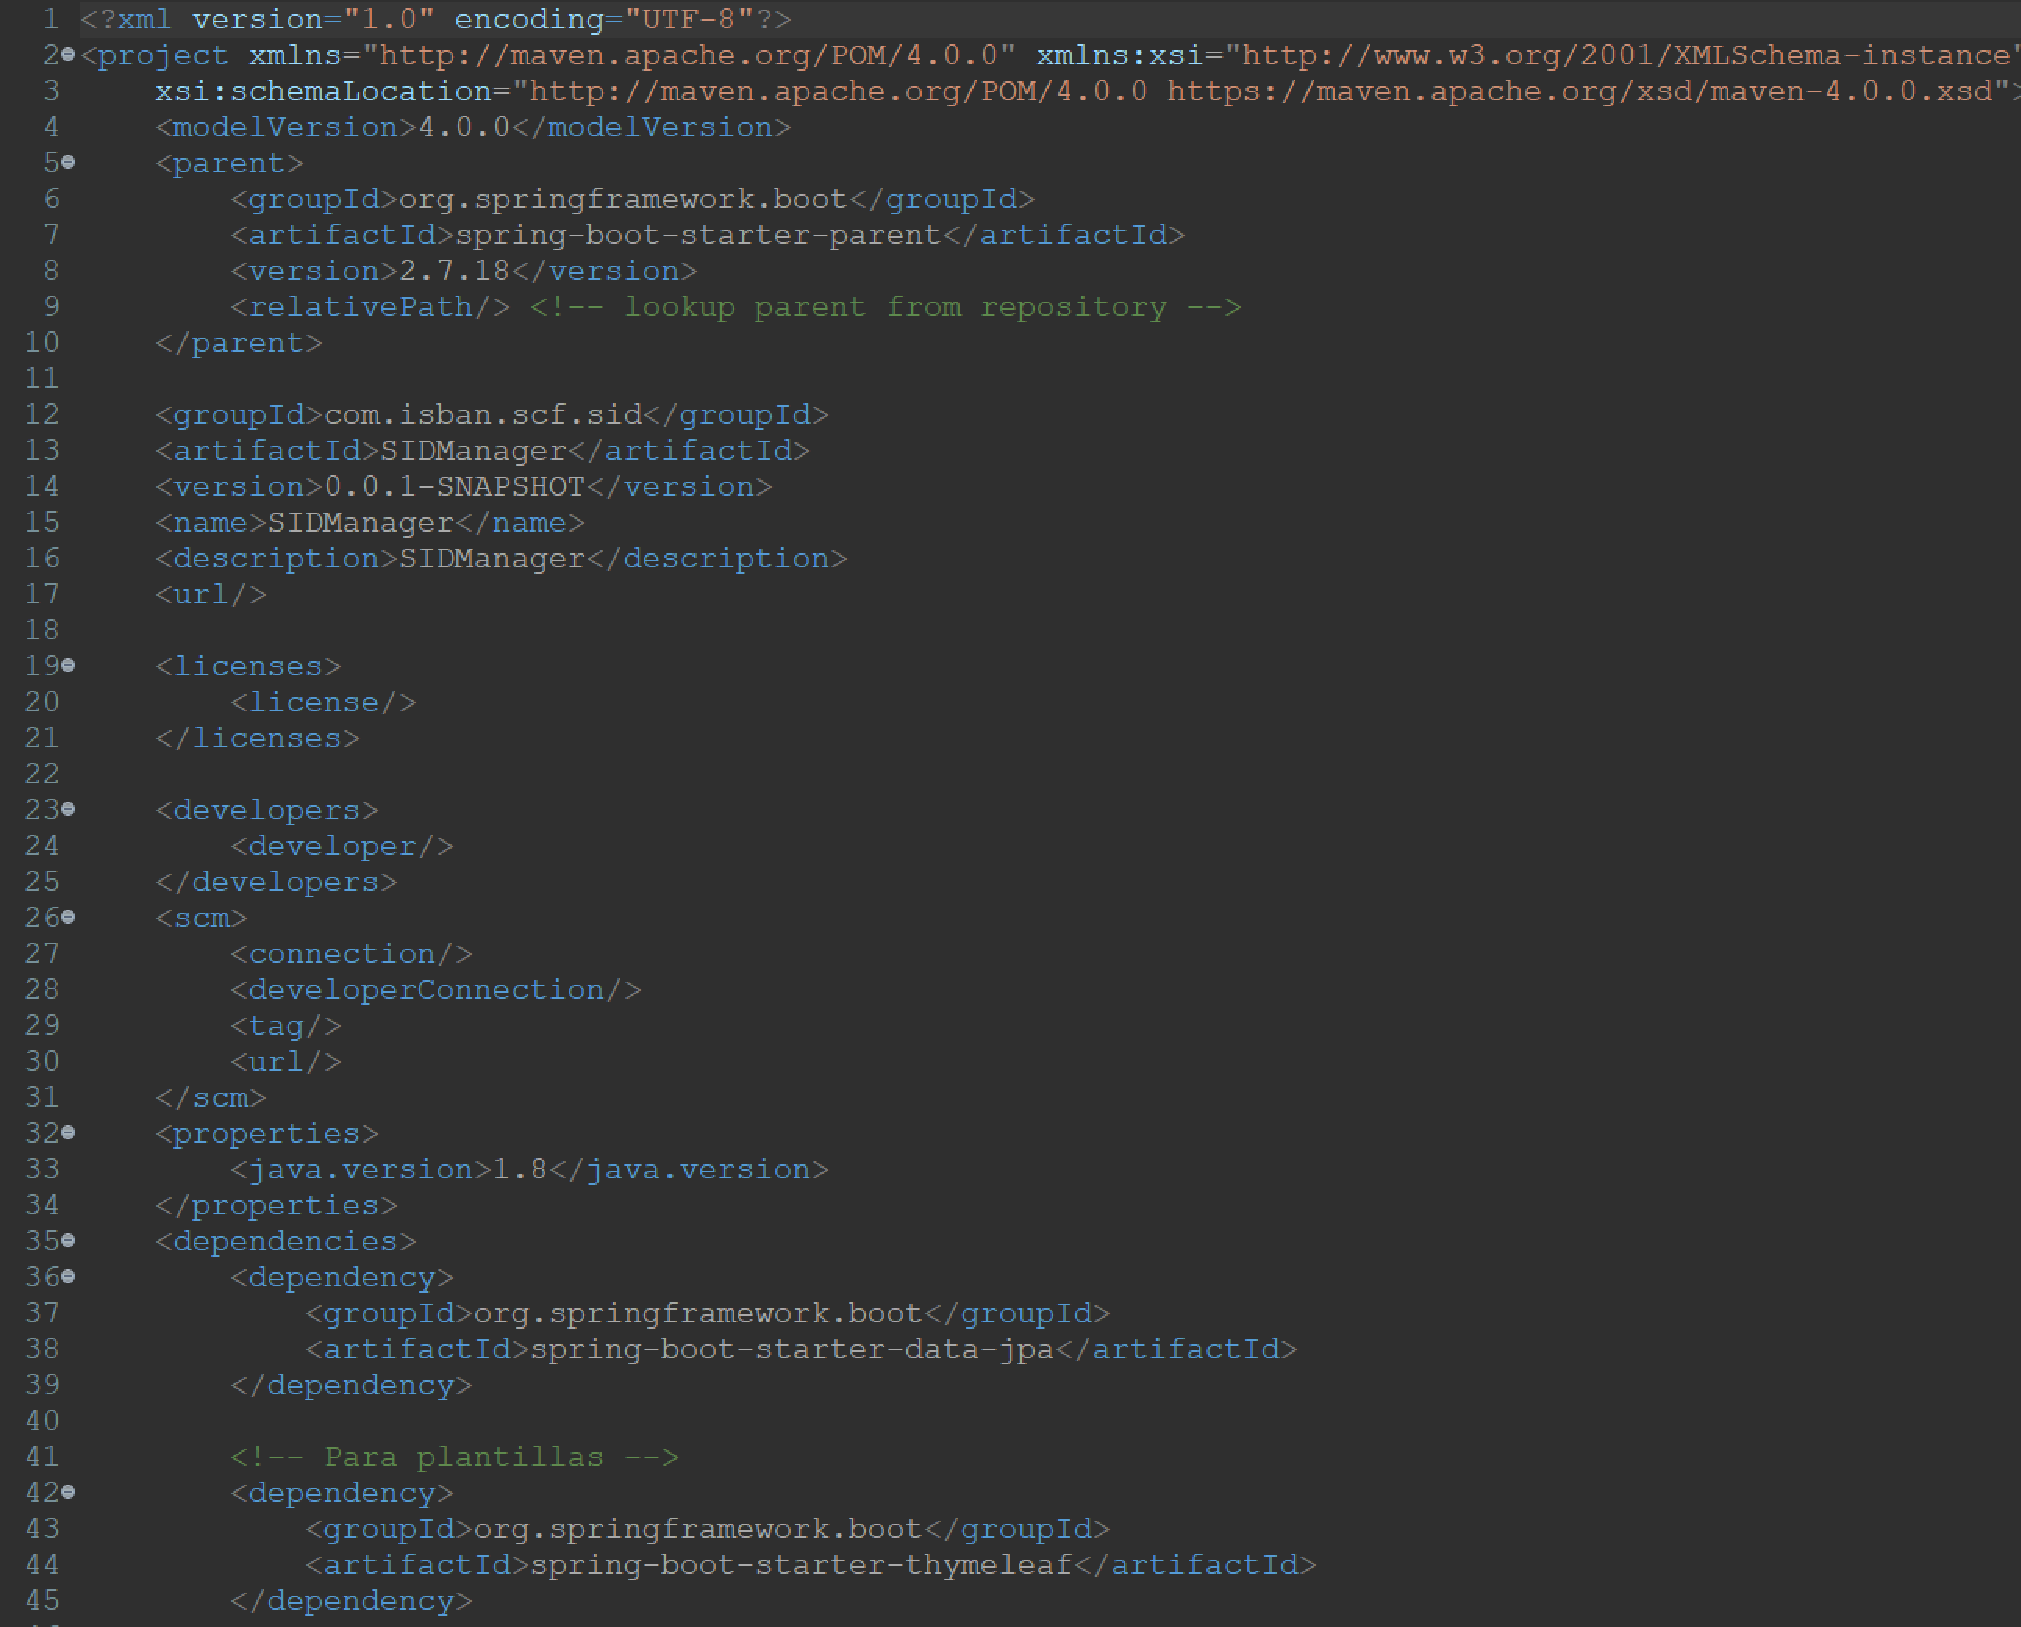
\includegraphics[width=0.75\linewidth]{imagenes/code/maven_pom_xml_example.pdf}
%     \caption{Archivo pom.xml de Maven del proyecto}
%     \label{fig:maven_pom}
% \end{figure}

% \subsection{Dependencias principales}

% A continuación, se describen las principales dependencias empleadas en el proyecto y su propósito:

% \begin{enumerate}
%     \item Thymeleaf:
%     Es un motor de plantillas que permite integrar datos dinámicos en las vistas HTML. Para más información, lea el apartado \ref{subsec:thymeleaf}.

%     \item MySQL Connector:
%     Este conector es la biblioteca que permite la conexión entre la aplicación Java y la base de datos MySQL. Es fundamental para realizar operaciones de consulta, inserción, actualización y eliminación en la base de datos.

%     \item javax.mail:
%     Biblioteca utilizada para la implementación de funcionalidades de envío de correos electrónicos. En este proyecto, se emplea para enviar correos de confirmación a los usuarios registrados, asegurando una validación adecuada de sus cuentas.

%     \item Javadoc:
%     Javadoc es una herramienta incluida en el JDK que permite generar documentación de las clases y métodos del proyecto a partir de comentarios en el código fuente. Esto facilita la comprensión y el mantenimiento del sistema.

%     \item Log4j:
%     Log4j es una biblioteca para la gestión de bitácoras (logs). Se utiliza para registrar eventos, errores y mensajes informativos durante la ejecución de la aplicación, lo que es crucial para la depuración y monitorización.

% \end{enumerate}



% \section{ API de gestión de documentos}

% Para poder hablar de la API, es importante hacer una distinción entre las dos partes principales de la aplicación: por un lado, la gestión de documentos, y por otro, la gestión de usuarios.

% En este apartado, se va a hablar de la gestión de documentos, es decir, de cómo funciona la aplicación por dentro para mostrar por pantalla el listado con las características de los documentos.

% Encontramos tres funciones principales en el controlador: getAllDocuments, getNotReceivedDocuments y listDocuments.


% \subsection{ Función getAllDocuments }
% Esta función llama al método \emph{getAllDocuments} del servicio \emph{DocumentService} y devuelve la respuesta. El código de la función \emph{getAllDocuments}, junto con sus logs asociados, es el siguiente:

% \begin{lstlisting}[language=Java]
% @GetMapping()
% public String getAllDocuments(Model model) {
%     logger.debug(" ----- Entering getAllDocuments ----- ");
%     model.addAttribute("documents", documentService.getAllDocuments());
%     logger.debug(" ----- Exiting getAllDocuments ----- ");
%     logger.debug(" ____________________________________ ");
%     return "documentsView"; 
% }
% \end{lstlisting}

% Una vez en el método \emph{getAllDocuments} del \emph{DocumentService}, este llama a la función \emph{findAll} del \emph{DocumentRepository}, que es el repositorio encargado de interactuar con la base de datos. El código es el siguiente:

% \begin{lstlisting}[language=Java]
% public List<Document> getAllDocuments() {
%     logger.debug(" Entering findAllDocuments ");
%     return documentRepository.findAll();
% }
% \end{lstlisting}

% Gracias a JPA, la sintaxis utilizada (\emph{findAll}) permite generar automáticamente la consulta SQL sin necesidad de que el programador escriba la consulta explícitamente en el \emph{DocumentRepository}. Esto no solo ahorra tiempo, sino que también reduce la posibilidad de errores y mejora la claridad del código. Para una mejor comprensión, se recomienda revisar la figura \ref{fig:jpa-usage}.

% Más adelante, en la sección \ref{sec:jpa-sintaxis}, se explicará con más detalle el uso de JPA.

% En resumen, esta función devuelve todos los documentos de la base de datos, sin restricciones ni filtros aplicados, junto con sus respectivos datos asociados (tal como se explicó en la sección de arquitectura de los documentos \ref{subsec:document-architecture}).

    
% \textbf { \subsection { Función getNotReceivedDocuments }}
%     Esta función llama al método \emph{getNotReceivedDocuments} del servicio \emph{DocumentService} y devuelve la respuesta. El código de la función \emph{getNotReceivedDocuments}, junto con sus logs asociados, se puede observar en el anexo \ref{code:not-received-controller}.

% Una vez en el método \emph{getNotReceivedDocuments} del \emph{DocumentService}, este llama a la función \emph{findByReceivedAtIsNull} del \emph{DocumentRepository}. El código se puede observar en el anexo \ref{code:not-received-service}.



% En resumen, esta función devuelve todos los documentos de la base de datos que no hayan sido guardados correctamente, ya que no tienen fecha en el apartado \emph{received\_at} (para más información sobre la arquitectura del documento, ver la sección \ref{subsec:document-architecture}), por lo que no han sido recibidos. 

    
%     \textbf { \subsection { Función listDocuments}}

% La función \emph{listDocuments} es una de las piezas clave de la aplicación, ya que se encarga de recuperar y filtrar los documentos almacenados en la base de datos según un intervalo de fechas. Esta función combina dos métodos principales del servicio \emph{DocumentService}: \emph{checkDates} y \emph{getFilteredDocuments}. Para una primera comprensión de la función, se puede visualizar el diagrama de secuencia UML del apartado de diseño \ref{fig:list-documents-uml-diagram}. A continuación, se describe en detalle su funcionamiento y los componentes involucrados.


% La función \emph{listDocuments} realiza principalmente tres tareas: validación y ajuste de fecha, filtrado de documentos y preparación de la respuesta.
% A través del método \emph{checkDates}, se valida y ajusta el intervalo de fechas proporcionado por el usuario. Este intervalo se almacena en una clase auxiliar llamada \emph{DateRange}, que encapsula las fechas de inicio y fin para facilitar su manejo entre métodos.
% Utilizando el intervalo de fechas validado, se invoca el método \emph{getFilteredDocuments} para recuperar los documentos que cumplen con el criterio de filtrado.
% Finalmente, la función añade al modelo (\emph{model}) los documentos filtrados, junto con las fechas de inicio y fin utilizadas en el filtrado. Esta información se envía a la vista para su visualización.


% El código de la función \emph{listDocuments}, junto con sus logs asociados, se puede apreciar en el anexo \ref{code:list-docs}.


% Una vez que el intervalo de fechas ha sido validado, la función \emph{listDocuments} invoca el método \emph{getFilteredDocuments} del servicio \emph{DocumentService}. Este método, a su vez, llama a una función del repositorio \emph{DocumentRepository} para ejecutar la consulta SQL que filtra los documentos según las fechas proporcionadas. Se puede consultar el código en el anexo \ref{code:list-docs-service}.


% Dado que esta consulta es específica y no se ajusta a las convenciones automáticas de JPA, se ha implementado manualmente en el repositorio utilizando una anotación \emph{@Query}. La consulta SQL correspondiente se puede ver en el código del repositorio que está en el anexo \ref{code:list-docs-repositoty}.



% Método \emph{checkDates}

% El método \emph{checkDates} desempeña un papel crucial en la función \emph{listDocuments}, ya que se encarga de validar y ajustar las fechas proporcionadas por el usuario. Su implementación responde a tres necesidades principales: validación de errores, pseudopaginación y manejo de casos especiales.
% Respecto a la validación de errores, esta garantiza que las fechas proporcionadas sean válidas y estén en el formato correcto. Si no se realiza esta validación, errores en las fechas podrían interrumpir el funcionamiento de la aplicación.
% Por otro lado, en entornos de preproducción, se observó que la carga de más de 80.000 documentos podía tardar entre 6 y 8 minutos. Para optimizar el rendimiento, se implementó una pseudopaginación que limita el intervalo de fechas a un máximo de 10 días. Este límite se estableció tras un análisis exhaustivo que demostró que, a partir de este número, el tiempo de carga comenzaba a ser demasiado largo (3 segundos).
% Finalmente, el método gestiona situaciones en las que el usuario no proporciona ambas fechas o cuando el intervalo de fechas excede el límite establecido; en este caso, el límite es de 10 días como se ha comentado anteriormente.

% El código del método \emph{checkDates} se puede apreciar en el anexo \ref{code:checkDates}.



% El método \emph{checkDates} está diseñado para manejar cinco escenarios principales:

% \begin{itemize}
%     \item Ambas fechas proporcionadas: Si las fechas son válidas y el intervalo no excede los 10 días, se devuelve el intervalo original. En caso contrario, se ajusta el intervalo a los últimos 10 días y se notifica al usuario.
    
%     \item Solo la fecha de fin proporcionada: Se calcula un intervalo de 10 días hacia atrás a partir de la fecha de fin.
    
%     \item Solo la fecha de inicio proporcionada: Se calcula un intervalo de 10 días hacia adelante a partir de la fecha de inicio.
    
%     \item Ninguna fecha proporcionada: Se devuelve un intervalo predeterminado de los últimos 10 días.
    
%     \item Error en el formato de las fechas: Si ocurre un error al parsear las fechas, se devuelve un intervalo predeterminado y se registra el error.
% \end{itemize}


% En resumen, la función \emph{listDocuments} permite recuperar documentos filtrados por un intervalo de fechas, optimizando el rendimiento mediante la pseudopaginación y garantizando la robustez del sistema mediante la validación de entradas. Este enfoque no solo mejora la experiencia del usuario, sino que también asegura un manejo eficiente de grandes volúmenes de datos.


% \section{ API de gestión de usuarios}
% En lo que respecta a la gestión de usuarios, encontramos tres apartados principales (proceso de registro, inicio de sesión y cambio de contraseña) en los que se agrupan las distintas funciones del controlador ClientController. Estos apartados son: registro de usuarios, inicio de sesión y cambio de contraseña.

% % Sign Up
%  \subsection{ Registro de usuarios (signup) }
% El proceso de registro en la aplicación SIDManager consta de tres pasos (o funciones). El primero es la carga de la página de registro, el segundo es el proceso de registrarse y el tercero es la confirmación del usuario a través del correo electrónico. Estos tres pasos se corresponden a tres funciones distintas: getCreateClientUserView, createClientUser, getConfirmation. Las funciones están detalladas a continuación:


% \begin{enumerate}
%     \item  Función getCreateClientUserView

    
%     Esta función devuelve la vista (o página) del proceso de registro del usuario. La función en el ClientController se encuentra en el anexo \ref{code:getCreateClientUserView}.

%     Esta función devuelve la vista ante la petición GET del usuario para poder comenzar el registro. Después de rellenar los campos del registro (correo electrónico, contraseña y contraseña repetida) con los datos del usuario y de pulsar el botón "sign up" se llama a la función createClientUser.
    

%   \item  Función createClientUser

% La función \emph{createClientUser} es la encargada de gestionar el proceso de registro de un nuevo usuario en la aplicación. Esta función recibe los datos del formulario de registro, valida la información y, si todo es correcto, guarda al usuario en la base de datos y envía un correo electrónico de confirmación. Para una primera comprensión de la función, se puede visualizar el diagrama de secuencia UML del apartado de diseño \ref{fig:sign-up-uml-diagram}. Para ver el código, consulta el anexo \ref{code:createClientUser-controller}.


% Los parámetros de entrada son los siguientes:
%     \begin{itemize}
%         \item \emph{Model model}: Se utiliza para pasar datos a la vista, como mensajes de respuesta o errores.
%         \item \emph{@ModelAttribute ClientUser clientUser}: Contiene los datos del usuario proporcionados en el formulario de registro (correo electrónico y contraseña).
%         \item \emph{@RequestParam("psw-repeat") String passwordRepeat}: Contiene la contraseña repetida para verificar que coincida con la contraseña original.
%     \end{itemize}

%     Lógica del controlador:
%     La función llama al método \emph{createClientUser} del servicio \emph{ClientUserService}, pasando los datos del usuario y la contraseña repetida.
%     Dependiendo del resultado del servicio, se añade un mensaje de respuesta al modelo (\emph{model}) para informar al usuario sobre el éxito o el fracaso del registro.
%     Finalmente, se devuelve la vista \emph{createClientUserView}, que muestra el formulario de registro junto con el mensaje de respuesta.


%      \item  Función \emph{saveClientUser}

% La función \emph{saveClientUser} es la encargada de guardar un nuevo usuario en la base de datos. Esta función realiza varias operaciones críticas, como la encriptación de la contraseña, la generación de un código de confirmación único y la asignación de un estado inicial al usuario. Se puede ver la función en el anexo \ref{code:saveClientUser-controller}.

%     En primer lugar, la contraseña proporcionada por el usuario se encripta utilizando la función \emph{encryptFacade}. Esto garantiza que la contraseña no se almacene en texto plano en la base de datos, mejorando la seguridad del sistema. Para más información sobre la encriptación, ver la sección \ref{sec:cryptography}.

%     Por otro lado, se genera un código de confirmación único utilizando \emph{RandomStringUtils.randomAlphanumeric(30)}. Este código se enviará al usuario por correo electrónico y se utilizará para confirmar su registro.

%     Además de lo anterior, el estado del usuario se establece en \emph{0}, lo que indica que el usuario ha sido creado pero aún no ha confirmado su correo electrónico. Mientras tenga su estado en 0, no podrá iniciar sesión, por lo que tendrá que confirmar al usuario abriendo el correo con el enlace proporcionado para ello.

%     También se registra la fecha y hora actuales como la fecha de creación del usuario.

%     Finalmente, el usuario se guarda en la base de datos utilizando el método \emph{save} del repositorio \emph{clientUserRepository}.

%     Si ocurre algún error durante el proceso (por ejemplo, si la contraseña es nula), se lanza una excepción y se registra el error en los logs.

% Las funciones explicadas anteriormente trabajan juntas para garantizar un proceso de registro seguro y eficiente.
% Primeramente, respecto a la validación de datos, la función \emph{createClientUser} valida que las contraseñas coincidan y que el correo electrónico no esté ya registrado en la base de datos.
% Además de lo anterior, la función \emph{saveClientUser} se encarga de encriptar la contraseña, generar un código de confirmación único y guardar al usuario en la base de datos.
% Una vez que el usuario se ha guardado correctamente, se envía un correo electrónico con el código de confirmación para que el usuario pueda activar su cuenta.
% Para finalizar, el controlador devuelve un mensaje de respuesta a la vista, informando al usuario sobre el éxito o el fracaso del registro.
    

% Las funciones comentadas son fundamentales para el proceso de registro en la aplicación SIDManager. Juntas, garantizan que los datos del usuario se validen, almacenen de manera segura y se confirmen a través de un correo electrónico. Este enfoque no solo mejora la seguridad del sistema, sino que también proporciona una experiencia de usuario fluida y confiable.
    
%     \item Función getConfirmation

% Antes de explicar la función \emph{getConfirmation}, es importante recordar que un usuario, al crearse, tiene un estado inicial de \emph{0} (creado pero no confirmado). Para confirmar su cuenta, se le envía un correo electrónico con un enlace único que lo redirige a una página de confirmación. Esta página cambia su estado a \emph{1} (confirmado) una vez que el usuario accede al enlace. La función \emph{getConfirmation} en el \emph{UserController} es la encargada de gestionar este proceso. Para ver el código de la función, consultar \ref{code:getConfirmation-controller}.


% Explicación del código \emph{getConfirmation}

% Los parámetros de entrada son:
%     \begin{itemize}
%         \item Model model: Se utiliza para pasar datos a la vista, como mensajes de respuesta o errores.
%         \item @RequestParam(''email'') String email: Contiene el correo electrónico del usuario que se está confirmando.
%         \item @RequestParam(''confirmationCode'') String confirmationCode: Contiene el código de confirmación único asociado al usuario.
%     \end{itemize}

% Por otro lado, respecto a la lógica del controlador, la función getConfirmation llama al método \emph{confirmUser} del servicio \emph{ClientUserService}, pasando el correo electrónico y el código de confirmación. Dependiendo del resultado del servicio, se añade un mensaje de respuesta al modelo (\emph{model}) para informar al usuario sobre el éxito o el fracaso de la confirmación. Finalmente, se devuelve la vista \emph{confirmationUser}, que muestra el resultado de la confirmación.


% El código de la función \emph{confirmUser} se encuentra en el anexo \ref{code:confirmUser-service}.


% Primeramente, en \emph{confirmUser} se realiza la búsqueda del usuario, es decir, se busca en la base de datos un usuario que coincida con el correo electrónico, el código de confirmación y tenga un estado de \emph{0} (no confirmado). Esto se realiza mediante la función \emph{findByEmailAndConfirmationCodeAndStatus} del repositorio \emph{clientUserRepository}.
% Cabe destacar también la confirmación del usuario, es decir, si se encuentra un usuario que cumple con los criterios, se cambia su estado a \emph{1} (confirmado) y se registra la fecha y hora de confirmación.
% El usuario actualizado se guarda en la base de datos utilizando el método \emph{save} del repositorio.
% Y por último se devuelve un mensaje de éxito (\emph{ResponseEnum.CONFIRM\_SUCCESS}).
    
% Si no se encuentra un usuario que cumpla con los criterios (por ejemplo, si el usuario ya está confirmado o el código de confirmación es incorrecto), se devuelve un mensaje de advertencia (\emph{ResponseEnum.CONFIRM\_WARNING}).

% La función \emph{getConfirmation} y su correspondiente método en el servicio, \emph{confirmUser}, trabajan juntos para garantizar que el proceso de confirmación del usuario sea seguro y eficiente:

% \begin{itemize}
%     \item Acceso al enlace de confirmación:
%     El usuario accede al enlace único enviado por correo electrónico, que contiene su correo electrónico y código de confirmación.
    

%     \item Validación del usuario:
%     El sistema verifica que el correo electrónico y el código de confirmación coincidan con un usuario no confirmado en la base de datos.
    

%     \item Confirmación y actualización:
%     Si la validación es exitosa, el estado del usuario se cambia a \emph{1} (confirmado) y se registra la fecha de confirmación.
    

%     \item Retroalimentación al usuario:
%     El sistema muestra un mensaje en la vista \emph{confirmationUser} para informar al usuario sobre el resultado del proceso.
    
% \end{itemize}


% Por tanto, la función \emph{getConfirmation} y su método asociado \emph{confirmUser} son fundamentales para completar el proceso de registro en la aplicación SIDManager. Juntos, garantizan que solo los usuarios que hayan verificado su correo electrónico puedan activar sus cuentas, lo que mejora la seguridad y la confiabilidad del sistema. Este enfoque también proporciona una experiencia de usuario fluida, ya que el proceso de confirmación es rápido y sencillo.

% \end{enumerate}
    

% % Login
% \subsection{Inicio de sesión (login)}

% El proceso de inicio de sesión en la aplicación SIDManager es una de las funcionalidades más críticas, ya que garantiza que solo los usuarios autorizados puedan acceder al sistema. Inicialmente, este proceso se implementó de manera manual, pero debido a consideraciones de seguridad, se migró a una solución basada en Spring Boot Security. Por tanto, si quiere saber aspectos avanzados del inicio de sesión, consulte la sección \ref{sec:spring-security}. 

% La función \emph{getLoginView} es la encargada de preparar y devolver la vista de inicio de sesión. Esta función configura las URLs necesarias para acciones como la recuperación de contraseña y el registro de nuevos usuarios, además de manejar mensajes de error que puedan haberse generado en intentos previos de inicio de sesión. Para ver el código de la función, acceder al anexo \ref{code:getLoginView-controller}.


% \begin{enumerate}
%     \item La función getLoginView tiene dos parámetros de entrada. El primero es el \emph{Model model}, que se utiliza para pasar datos a la vista, como URLs y mensajes de error. El segundo es \emph{HttpServletRequest request}, el cual permite acceder a la sesión del usuario y recuperar atributos almacenados, como mensajes de error.
    

%     \item Configuración de URLs:
%     Se obtiene la URL base del servidor (\emph{serverUrl}) desde las propiedades compartidas (\emph{SharedProperties}).
%      Se construyen las URLs para la recuperación de contraseña (\emph{requestUpdatePasswordUrl}) y el registro de nuevos usuarios (\emph{createClientUserUrl}).
%       Estas URLs se añaden al modelo para que estén disponibles en la vista.
    

%     \item Manejo de mensajes de error:
%     Se verifica si hay un mensaje de error almacenado en la sesión del usuario (\emph{request.getSession().getAttribute("error")}).
%      Si existe un mensaje de error, se añade al modelo para mostrarlo en la vista. Además, se elimina el mensaje de la sesión para evitar que se muestre en futuras cargas de la página.
    

%     \item Retorno de la vista:
%     La función devuelve la vista \emph{loginView}, que muestra el formulario de inicio de sesión junto con las URLs configuradas y los mensajes de error, si los hay.
    
% \end{enumerate}


% La función \emph{getLoginView} es esencial para cargar la vista de inicio de sesión y configurar los elementos necesarios, como las URLs de recuperación de contraseña y registro. Además, maneja mensajes de error para mejorar la experiencia del usuario. La migración a Spring Boot Security ha fortalecido la seguridad del proceso de inicio de sesión, garantizando que solo los usuarios autorizados puedan acceder al sistema de manera segura.

% % Update psw
% \subsection{Cambio de contraseña (update password)}
% \label{subsec:update-password}

% El proceso de cambio de contraseña en la aplicación SIDManager es una funcionalidad crítica que garantiza la seguridad de los usuarios al permitirles actualizar sus credenciales de acceso. Este proceso consta de cuatro pasos principales, cada uno implementado mediante funciones específicas en el controlador y el servicio. A continuación, se describen en detalle estas funciones y su funcionamiento.

% \begin{enumerate}

%     \item   Función getRequestUpdatePasswordView

% La función getRequestUpdatePasswordView es la encargada de cargar la vista donde el usuario puede solicitar un cambio de contraseña. Esta vista incluye un formulario para ingresar el correo electrónico asociado a la cuenta. Se puede ver la función en el anexo \ref{code:getRequestUpdatePasswordView-controller}.

% La función responde a una solicitud HTTP GET en la ruta /user/requestUpdatePassword y devuelve la vista requestUpdatePasswordView, que contiene el formulario para solicitar el cambio de contraseña.


%     \item Función requestUpdatePassword

% Una vez que el usuario ingresa su correo electrónico y envía el formulario, se invoca la función requestUpdatePassword. Esta función valida el correo electrónico y, si es válido, envía un enlace único al usuario para que pueda cambiar su contraseña.  Se puede ver la función en el anexo \ref{code:requestUpdatePassword-controller}.



% Primero, la función responde a una solicitud HTTP POST en la ruta /user/requestUpdatePassword que recibe el correo electrónico del usuario como parámetro.
% Después llama al método sendUpdatePasswordUrl del servicio ClientUserService para validar el correo electrónico y enviar el enlace de cambio de contraseña.
% Además, la función añade un mensaje de respuesta al modelo para informar al usuario sobre el resultado de la operación.
% Por último, devuelve la vista requestUpdatePasswordView para mostrar el mensaje de respuesta.


% Método sendUpdatePasswordUrl

% El método sendUpdatePasswordUrl es el encargado de generar y enviar el enlace de cambio de contraseña al correo electrónico del usuario. Para ver el código de la función, accede al anexo \ref{code:sendUpdatePasswordUrl-service}.


% Primeramente, el sistema busca al usuario en la base de datos utilizando el correo electrónico proporcionado como criterio de búsqueda. A continuación, si el usuario existe y su cuenta está debidamente confirmada (lo que se verifica comprobando que su estado sea igual a 1), el procedimiento genera un enlace único mediante el método getConfirmationUrl, diseñado específicamente para cada usuario con el confirmationCode. Acto seguido, este enlace se envía al correo electrónico del usuario utilizando la clase Mail, la cual se encarga de gestionar el asunto, el cuerpo del mensaje y la incorporación del enlace (para un análisis detallado de la clase Mail, véase la sección \ref{subsec:mail}). Finalmente, el sistema devuelve un mensaje de éxito si la operación se completa correctamente o, en caso contrario, una notificación de advertencia que alerta sobre cualquier incidencia durante el proceso.


% El método getConfirmationUrl genera la URL de confirmación o cambio de contraseña utilizando la URL base del servidor y los datos del usuario. Se puede ver la función en el anexo \ref{code:getConfirmationUrl-service}.



% Por tanto, el método getConfirmationUrl construye una URL utilizando la URL base del servidor, el correo electrónico del usuario y su código de confirmación. La URL base se obtiene de las propiedades compartidas (SharedProperties), lo que permite cambiar la URL fácilmente sin modificar el código. Para más información sobre la clase SharedProperties, ver \ref{subsec:shared-properties}.


%     \item Función getUpdatePasswordView

% Cuando el usuario accede al enlace de cambio de contraseña, se invoca la función getUpdatePasswordView. Esta función valida el enlace y carga la vista para cambiar la contraseña. Para ver el código de la función, accede al anexo \ref{code:getUpdatePasswordView-controller}.



% La función getUpdatePasswordView delega la validación del correo electrónico y el código de confirmación al método getUpdatePasswordView del servicio. Si la validación es exitosa, muestra el formulario para cambiar la contraseña. Sin embargo, si la validación falla, muestra un mensaje de error. Por último, almacena el correo electrónico en la sesión para su uso posterior (ya que la función updatePassword lo necesita).


% El método getUpdatePasswordView valida que el usuario exista y que el código de confirmación sea correcto. Se puede ver la función en el anexo \ref{code:getUpdatePasswordView-service}.


% El método getUpdatePasswordView busca al usuario en la base de datos utilizando el correo electrónico, el código de confirmación y el estado 1 (confirmado) usando la sintaxis de JPA. Como salida, devuelve un mensaje de éxito o advertencia dependiendo del resultado de la búsqueda.


%     \item Función updatePassword

% Finalmente, cuando el usuario envía el formulario de cambio de contraseña, se invoca la función updatePassword. Esta función valida las nuevas contraseñas y actualiza la contraseña en la base de datos. Para ver el código de la función, accede al anexo \ref{code:updatePassword-controller}.



% La función updatePassword recibe las nuevas contraseñas y valida que coincidan. También llama al método updatePassword del servicio para actualizar la contraseña en la base de datos. Por último, muestra un mensaje de éxito o error y redirige al usuario a la página de inicio de sesión si la operación es exitosa.


% El método updatePassword realiza la actualización de la contraseña en la base de datos. Se puede ver la función en el anexo \ref{code:updatePassword-service}.


% El método `updatePassword` realiza la actualización de la contraseña siguiendo un proceso estructurado. Primeramente, valida que las contraseñas coincidan y que el usuario exista en la base de datos para garantizar la integridad de la operación. Más adelante, en caso de cumplirse estas condiciones, procede a encriptar la nueva contraseña utilizando un facade de encriptación que le aplica BCrypt y la guarda en la base de datos actualizando el registro correspondiente. Para más información sobre encriptación, ver el apartado \ref{sec:cryptography}. Finalmente, devuelve un mensaje de éxito si la operación se completa correctamente o un mensaje de error en caso de que alguna validación falle, informando al usuario sobre el resultado del proceso.

% El proceso de cambio de contraseña en SIDManager es un ejemplo de cómo se puede implementar una funcionalidad crítica de manera segura y eficiente. Utilizando Spring Boot y buenas prácticas de desarrollo, se garantiza que los usuarios puedan actualizar sus credenciales de manera sencilla y segura, protegiendo así la integridad de sus cuentas.

% \end{enumerate}

% %\section{ Acceso a la base de datos mediante generación automática de consultas SQL con JPA}
% \section{ Generación automática de consultas SQL con JPA }
% \label{sec:jpa-sintaxis}
% En esta sección se explicará cómo JPA (Java Persistence API) construye automáticamente consultas SQL a partir de su propia sintaxis, simplificando enormemente la interacción con la base de datos. Para ilustrar este proceso, nos basaremos en el ejemplo mostrado en la figura \ref{fig:jpa-usage}, donde se utiliza el método \emph{findAll()}. Sin embargo, esto puede plantear una pregunta importante: ¿cómo sabe JPA que debe recuperar entidades de tipo \emph{Document} y no de otra entidad de la base de datos?

% La respuesta reside en la configuración de la clase \emph{DocumentRepository}, que actúa como interfaz entre la capa de persistencia y la lógica de negocio. A continuación, se muestra el fragmento de código clave:

% \begin{lstlisting}[language=Java]
% import com.isban.scf.sid.model.Document;

% @Repository
% public interface DocumentRepository extends JpaRepository<Document, Long> {
% \end{lstlisting}

% Explicación del código

% \begin{enumerate}
% \item Importación del modelo \emph{Document}:
% En la primera línea del código, se importa la clase \emph{Document}, que representa la entidad de la base de datos con la que se va a trabajar. Esta clase está anotada con \emph{@Entity} en su definición, lo que indica a JPA que se trata de una entidad persistente mapeada a una tabla en la base de datos.

% \item Uso de la anotación \emph{@Repository}: 
% La anotación \emph{@Repository} marca la interfaz \emph{DocumentRepository} como un componente de Spring encargado de la gestión de operaciones de persistencia. Esta anotación no solo permite que Spring detecte automáticamente esta clase durante el escaneo de componentes, sino que también proporciona manejo de excepciones específicas de persistencia.

% \item Extensión de \emph{JpaRepository}: 
% La interfaz \emph{DocumentRepository} extiende \emph{JpaRepository<Document, Long>}, lo que le proporciona acceso a una serie de métodos predefinidos para realizar operaciones CRUD (Crear, Leer, Actualizar y Eliminar) sobre la entidad \emph{Document}. El primer parámetro genérico (\emph{Document}) indica el tipo de entidad con la que se trabajará, mientras que el segundo parámetro (\emph{Long}) especifica el tipo de la clave primaria de dicha entidad.

% \item Generación automática de consultas: 
% Al extender \emph{JpaRepository}, JPA automáticamente implementa métodos como \emph{findAll()}, \emph{findById()}, \emph{save()}, entre otros, sin necesidad de escribir código adicional. En el caso de \emph{findAll()}, JPA genera la consulta SQL necesaria para recuperar todos los registros de la tabla asociada a la entidad \emph{Document}. Esto es posible gracias a la información proporcionada por los parámetros genéricos y las anotaciones de la entidad.

% \end{enumerate}



% El modelo \emph{Document} es una clase Java que representa la entidad documentos en la base de datos. Esta clase está mapeada a la tabla \emph{documents} mediante anotaciones de JPA, lo que permite a JPA realizar operaciones de persistencia de manera automática. En el anexo se puede ver el código de la clase \emph{Document} \ref{code:DocumentModel}.


% \begin{enumerate}
% \item Anotación \emph{@Entity}:
% Esta anotación indica que la clase \emph{Document} es una entidad JPA, lo que significa que está mapeada a una tabla en la base de datos.

% \item Anotación \emph{@Table}: 
% La anotación \emph{@Table(name = "documents")} especifica el nombre de la tabla en la base de datos a la que está asociada esta entidad. En este caso, la tabla se llama \emph{documents}.

% \item Campo \emph{clientDocId}: 
% Este campo está anotado con \emph{@Id} y \emph{@Column(name = ``CLIENT\_DOC\_ID``)}. El tipo de dato es \emph{Long}, y su valor identifica de manera única cada documento en la base de datos.

% \item Campo \emph{clientAppId}: 
% Este campo está anotado con \emph{@Column(name = ``CLIENT\_APP\_ID``)} y representa el identificador de la aplicación cliente que creó el documento. Su tipo de dato es \emph{Long}.

% \item Campo \emph{providerId}: 
% Este campo está anotado con \emph{@Column(name = ``PROVIDER\_ID``)} y almacena el identificador del proveedor que procesa el documento. Su tipo de dato es \emph{String}.

% \item Campos \emph{sentAt} y \emph{receivedAt}: 

% Estos campos están anotados con \text{@Column(name = ``SENT\_AT``)} y \text{@Column(name = ``RECEIVED\_AT``)}, respectivamente. 
% Representan las fechas en las que el documento fue enviado al proveedor y recibido de vuelta en la base de datos. Ambos campos son de tipo \emph{String}.

% \item Getters y setters: 
% Los métodos \emph{get} y \emph{set} permiten acceder y modificar los valores de los campos de la entidad. Estos métodos son esenciales para que JPA pueda interactuar con los datos de la entidad.

% \end{enumerate}


% La clave para que JPA sepa qué entidad debe utilizar reside en los parámetros genéricos de \emph{JpaRepository}. Al especificar \emph{Document} como el tipo de entidad, JPA vincula automáticamente esta interfaz con la tabla de la base de datos correspondiente a la entidad \emph{Document}. Además, la anotación \emph{@Entity} en la clase \emph{Document} proporciona los metadatos necesarios para realizar este mapeo, como el nombre de la tabla y las columnas.

% Este enfoque no solo reduce la cantidad de código repetitivo, sino que también garantiza que las consultas generadas sean consistentes y optimizadas para la entidad específica. Además, al utilizar métodos predefinidos como \emph{findAll()}, se minimiza el riesgo de errores sintácticos en las consultas SQL, ya que JPA se encarga de generarlas de manera automática y segura.


% \subsection{Ejemplo avanzado de sintaxis JPA}
% \label{subsec:ejemplo-avanzado-jpa }

% En el ejemplo anterior, se mostró cómo JPA convierte automáticamente el método \emph{findAll()} en una consulta SQL para recuperar todos los registros de una tabla. Sin embargo, este ejemplo es bastante básico y no refleja completamente la potencia y simplicidad que ofrece JPA para construir consultas más complejas. Para ilustrar mejor estas capacidades, analizaremos un caso más avanzado en el que se busca un usuario en la base de datos utilizando múltiples criterios.

% Contexto del ejemplo
% En el servicio \emph{ClientService} existe una función que busca un usuario en la base de datos dado su correo electrónico (\emph{email}), su código de confirmación (\emph{confirmationCode}) y su estado (\emph{status}). Sin utilizar las capacidades avanzadas de JPA, esta funcionalidad podría implementarse de la siguiente manera:

% \begin{lstlisting}[language=Java]
% // Código en el servicio
% ClientUser clientUser = clientUserRepository.customFindByEmailAndConfirmationCodeAndStatus(
% email, confirmationCode, 1
% );

% // Código en el repositorio
% @Query(value = "SELECT * FROM client_user WHERE email = ?1 AND confirmation_code = ?2 AND status = ?3", nativeQuery = true)
% ClientUser customFindByEmailAndConfirmationCodeAndStatus(
% @Param("email") String email,
% @Param("confirmationCode") String confirmationCode,
% @Param("status") int status
% );
% \end{lstlisting}

% En este enfoque, se requieren tres líneas de código: una en el servicio para invocar el método y dos en el repositorio para definir la consulta SQL personalizada. Aunque funcional, este método implica escribir código adicional y aumenta el riesgo de errores sintácticos o lógicos al manejar consultas SQL manualmente.

% Solución con JPA
% JPA ofrece una sintaxis avanzada que permite generar consultas automáticamente basándose en el nombre del método. Esto elimina la necesidad de escribir consultas SQL manualmente y reduce significativamente la cantidad de código necesario. Para el mismo caso, la implementación con JPA sería la siguiente:

% \begin{lstlisting}[language=Java]
% // Código en el servicio
% ClientUser clientUser = clientUserRepository.findByEmailAndConfirmationCodeAndStatus(
% email, confirmationCode, 1
% );
% \end{lstlisting}

% Explicación del código
% \begin{itemize}
% \item Nombre del método:

% El nombre del método \emph{findByEmailAndConfirmationCodeAndStatus} sigue una convención específica de JPA. JPA interpreta este nombre y genera automáticamente la consulta SQL correspondiente. 
% En este caso, la consulta buscará un registro en la tabla \emph{client\_user} donde los campos \emph{email}, \emph{confirmation\_code} y \emph{status} coincidan con los valores proporcionados.

% \item Parámetros del método: 
% Los parámetros \emph{email}, \emph{confirmationCode} y \emph{status} se pasan al método y se utilizan como criterios de búsqueda en la consulta generada.

% \item Resultado: 
% El método devuelve un objeto de tipo \emph{ClientUser} que cumple con los criterios especificados. Si no se encuentra ningún registro, el resultado será \emph{null}.

% \end{itemize}

% Ventajas de este enfoque

% \begin{itemize}
% \item Reducción de código repetitivo: Al utilizar métodos predefinidos de \emph{JpaRepository}, no es necesario escribir consultas SQL manualmente para operaciones comunes.
% \item Seguridad y consistencia: JPA garantiza que las consultas generadas sean seguras y consistentes con el modelo de datos.
% \item Facilidad de mantenimiento: Al centralizar la lógica de acceso a datos en repositorios, el código es más fácil de mantener y escalar.
% \item Integración con Spring: La anotación \emph{@Repository} permite una integración fluida con el contenedor de Spring, facilitando la inyección de dependencias y la gestión de transacciones.
% \end{itemize}



% \section{Integración del inicio de sesión con Spring Boot Security}
% \label{sec:spring-security}

% Inicialmente, el proceso de inicio de sesión en la aplicación SIDManager se implementó manualmente, lo que implicaba gestionar la autenticación y la autorización de los usuarios directamente en el código. Aunque esta aproximación funcionaba, presentaba varios riesgos de seguridad, como la posible exposición de credenciales, la falta de protección contra ataques comunes (por ejemplo, ataques de fuerza bruta) y la dificultad para mantener y escalar el código. Además, implementar manualmente todas las medidas de seguridad necesarias requería un conocimiento avanzado y un esfuerzo significativo.

% Para abordar estos problemas, se decidió migrar a una solución basada en Spring Boot Security, un framework robusto y ampliamente utilizado para gestionar la seguridad en aplicaciones Spring. Spring Boot Security proporciona mecanismos integrados para:

% \begin{itemize}
%     \item Autenticación: Verifica las credenciales del usuario (correo electrónico y contraseña) contra la base de datos.
%     \item Autorización: Controla el acceso a recursos específicos en función de los roles del usuario.
%     \item Protección contra ataques: Incluye medidas como el bloqueo de cuentas después de múltiples intentos fallidos, el cifrado de contraseñas y la protección contra ataques CSRF (Cross-Site Request Forgery).
% \end{itemize}

% La migración a Spring Boot Security no fue trivial, ya que implicó una serie de pasos técnicos complejos y la adaptación de la aplicación existente. A continuación, se describen los pasos clave que se siguieron para lograr una integración exitosa.

% \begin{enumerate}
%     \item Actualización de la vista
    
% Para que Spring Boot Security pueda detectar automáticamente los campos de entrada en el formulario de inicio de sesión, fue necesario actualizar la plantilla HTML de la vista. En particular, los campos del formulario deben seguir convenciones específicas. Por ejemplo, el campo de nombre de usuario debe tener el atributo name=''username'', y el campo de contraseña debe tener el atributo name=''password''. Esto permite que Spring Boot Security identifique y procese correctamente los datos del formulario.

% Este paso, aunque aparentemente sencillo, es crucial para garantizar que el framework pueda integrarse sin problemas con el front-end. Para más detalles, se puede consultar el tutorial oficial de Spring: \url{https://spring.io/guides/gs/securing-web#header}.

%     \item Implementación de la clase SecurityConfig
    
% El núcleo de la configuración de Spring Boot Security reside en la clase SecurityConfig. Esta clase define las reglas de seguridad, como las rutas que requieren autenticación, la página de inicio de sesión personalizada, el manejo de errores y el proceso de cierre de sesión (logout). En el anexo, se muestra la clase SecurityConfig implementada en SIDManager \ref{code:SecurityConfig}.



% La clase \emph{SecurityConfig} configura integralmente los aspectos de seguridad de la aplicación Spring Boot mediante una estructura jerárquica. Inicialmente, establece las reglas de autorización mediante \emph{authorizeHttpRequests}, donde se especifican las rutas públicas como \emph{/user/login}, \emph{/user/create} y recursos estáticos (\emph{/css/**}, \emph{/js/**}), mientras que el resto de los endpoints requiere autenticación.

% Para el proceso de autenticación, se implementa un formulario de login personalizado en \emph{/user/login} que, al tener éxito, redirige al usuario a \emph{/list}. Este flujo incorpora un manejador de fallos personalizado (\emph{CustomAuthenticationFailureHandler}) que gestiona los intentos fallidos de manera específica para la aplicación. El subsistema de logout está configurado para invalidar la sesión, eliminar cookies y redirigir a la página de login con un parámetro de confirmación.

% En el núcleo de seguridad, se emplea \emph{BCryptPasswordEncoder} como algoritmo de hashing para contraseñas, proporcionando un almacenamiento seguro de credenciales. La configuración se completa con un manejador de excepciones que redirige los accesos no autorizados a \emph{/user/accessDenied}, cerrando así el ciclo completo de gestión de accesos.

% La arquitectura sigue el principio de separación de preocupaciones, delegando el servicio de detalles de usuario (\emph{UserDetailsService}) mediante inyección de dependencias, mientras que los beans esenciales como el filtro de seguridad (\emph{SecurityFilterChain}) y el codificador de contraseñas se definen explícitamente para su uso en toda la aplicación.

%     \item Implementación de la clase UserDetailsService
    
% La clase UserDetailsService es fundamental en Spring Boot Security, ya que se encarga de cargar los detalles del usuario desde la base de datos durante el proceso de autenticación. En SIDManager, se implementó una clase personalizada llamada CustomUserDetailsService para adaptarse al modelo de usuario existente. Se puede ver la clase CustomUserDetailsService en el anexo \ref{code:CustomUserDetailsService}.


% El servicio \emph{CustomUserDetailsService} implementa la interfaz \emph{UserDetailsService} de Spring Security, funcionando como puente entre el modelo de usuarios de la aplicación y el sistema de autenticación. El núcleo de su funcionamiento reside en el método \emph{loadUserByUsername}, que realiza una búsqueda en la base de datos utilizando el correo electrónico como identificador único.

% Cuando se invoca este servicio durante el proceso de autenticación, primero consulta el repositorio \emph{ClientUserRepository} para localizar al usuario correspondiente. Si la búsqueda no produce resultados, inmediatamente lanza una excepción \emph{UsernameNotFoundException}, interrumpiendo el flujo de autenticación e informando adecuadamente al sistema de seguridad.

% Para los casos exitosos, el servicio transforma la entidad \emph{ClientUser} en una instancia de \emph{CustomUserDetails}, que implementa la interfaz \emph{UserDetails} requerida por Spring Security. Esta adaptación permite integrar perfectamente el modelo de dominio de la aplicación con el framework de seguridad, manteniendo separación de preocupaciones y permitiendo la extensión futura de los detalles de usuario.

% La implementación sigue el patrón de inyección de dependencias, recibiendo el repositorio de usuarios a través del constructor, lo que facilita las pruebas unitarias y el mantenimiento del código. Este diseño asegura que la lógica de autenticación pueda evolucionar independientemente del mecanismo de persistencia subyacente.


%     \item Cambió en la manera de encriptar
    
% Con la migración a Spring Boot Security, se adoptó el uso de \emph{BCryptPasswordEncoder} para encriptar las contraseñas. Este método de encriptación es ampliamente recomendado debido a su seguridad y resistencia a ataques de fuerza bruta. Durante el proceso de registro o cambio de contraseña, las contraseñas se encriptan utilizando este encoder antes de almacenarlas en la base de datos. Para más detalles, consultar el apartado \ref{sec:cryptography}.

%     \item Modificación del UserDetailsService a uno personalizado
    
% Para integrar completamente el sistema de autenticación de Spring Boot Security con el modelo de usuario de SIDManager, fue necesario implementar una clase personalizada que extendiera \emph{UserDetailsService}. Esta clase, \emph{CustomUserDetailsService}, se encarga de cargar los detalles del usuario desde la base de datos y adaptarlos a la interfaz requerida por Spring Boot Security. Este paso fue crucial para garantizar que el sistema de autenticación funcionara correctamente con el modelo de usuario existente. Se puede ver la clase CustomUserDetailsService en el anexo \ref{code:CustomUserDetailsService-modified}.


%     \item CustomAuthenticationFailureHandler

% Durante el proceso de autenticación, es crucial manejar adecuadamente los errores que puedan ocurrir, como credenciales incorrectas o cuentas bloqueadas. Para personalizar este manejo de errores, se implementó la clase \emph{CustomAuthenticationFailureHandler}, que extiende la interfaz \emph{AuthenticationFailureHandler} de Spring Boot Security. Esta clase permite controlar el flujo de la aplicación cuando un intento de inicio de sesión falla, proporcionando una experiencia de usuario más clara y segura. Para ver el código de la clase CustomAuthenticationFailureHandler, ir al anexo \ref{code:CustomAuthenticationFailureHandler}.


% El componente \emph{CustomAuthenticationFailureHandler} implementa la interfaz \emph{AuthenticationFailureHandler} de Spring Security, proporcionando un mecanismo personalizado para gestionar los fallos de autenticación. Cuando un intento de inicio de sesión no es válido, el método \emph{onAuthenticationFailure} se activa automáticamente, iniciando un flujo de manejo de errores estructurado.

% El proceso comienza almacenando un mensaje de error descriptivo en la sesión HTTP actual, lo que permite mantener esta información entre múltiples peticiones. Este mensaje, con el texto \emph{"Login error"}, puede ser recuperado posteriormente en la vista para informar al usuario sobre el problema específico ocurrido durante su intento de autenticación.

% Inmediatamente después de configurar el mensaje de error, el controlador ejecuta una redirección a la página de inicio de sesión original (\emph{/user/login}). Este enfoque garantiza que el usuario tenga la oportunidad de corregir sus credenciales mientras mantiene un flujo de navegación coherente. La implementación demuestra cómo extender el comportamiento predeterminado de Spring Security para crear experiencias de usuario más informativas y personalizadas, sin comprometer la seguridad del sistema.

% La implementación de \emph{CustomAuthenticationFailureHandler} es un ejemplo de cómo Spring Boot Security permite adaptar el comportamiento predeterminado para satisfacer las necesidades específicas de la aplicación. Este nivel de personalización es fundamental para garantizar que los usuarios reciban retroalimentación clara y útil en caso de errores, lo que contribuye a una experiencia de usuario más fluida y segura.


% \end{enumerate}


% La migración a Spring Boot Security ha sido un hito importante en el desarrollo de SIDManager, ya que ha permitido mejorar significativamente la seguridad de la aplicación. Aunque el proceso fue técnicamente desafiante, los beneficios obtenidos justifican el esfuerzo. Ahora, la aplicación cuenta con un sistema de autenticación y autorización robusto, protegido contra ataques comunes y fácil de mantener. Este logro demuestra cómo la combinación de buenas prácticas y herramientas modernas puede resolver problemas complejos en el desarrollo de software.


% \section{ Cifrado y seguridad }
% \label{sec:cryptography}
% En este apartado se definen los dos métodos de encriptación que tenemos (el que he desarrollado "Encyptor" y el de Spring Boot "PasswordEncoder") y cómo es que el cambio de uno a otro ha sido tan sencillo. Esto es debido a que se ha usado el patrón de software facade (fachada), ya que solo debemos especificar el método de encriptación en esta clase y cambiará para todas las funciones que usan la encriptación. La función que usa este patrón es:

% \begin{lstlisting}[language=java]
% public String encryptFacade(String password) {
%     //return Encryptor.encryptMessage(password);
%     return passwordEncoder.encode(password);
% }
% \end{lstlisting}

% \subsection{ Encriptación de contraseñas (PasswordEncoder) }
% \label{subsec:password-encoder}

% Uno de los aspectos más críticos en la seguridad de una aplicación es la gestión segura de las contraseñas de los usuarios. Para garantizar que las contraseñas se almacenen de manera segura, Spring Boot Security proporciona la interfaz \emph{PasswordEncoder}, que permite implementar algoritmos de encriptación robustos. En SIDManager, se ha utilizado \emph{BCryptPasswordEncoder}, un encoder ampliamente recomendado por su seguridad y resistencia a ataques.

% BCrypt tiene las siguientes especificaciones:

% \begin{itemize}
%     \item Algoritmo de hashing: BCrypt utiliza un algoritmo de hashing unidireccional, lo que significa que es prácticamente imposible revertir el proceso para obtener la contraseña original.
%     \item Salt automático: BCrypt genera automáticamente un valor de "salt" único para cada contraseña, lo que añade una capa adicional de seguridad al evitar que dos contraseñas idénticas produzcan el mismo hash.
%     \item Resistencia a ataques de fuerza bruta: Gracias a su diseño, BCrypt es resistente a ataques de fuerza bruta y de diccionario, ya que el proceso de hashing es intencionalmente lento y costoso computacionalmente.
%     \item Configuración de la fuerza de hashing: BCrypt permite ajustar la "fuerza" del hashing (número de rondas de procesamiento), lo que permite equilibrar la seguridad y el rendimiento según las necesidades de la aplicación.
% \end{itemize}

% \begin{lstlisting}[language=Java]
% @Bean
% public PasswordEncoder passwordEncoder() {
%     return new BCryptPasswordEncoder();
% }
% \end{lstlisting}



% El método \emph{passwordEncoder()}, anotado con @Bean, define un componente gestionado por Spring dentro del contexto de la aplicación. Este bean se encarga de proporcionar una instancia de BCryptPasswordEncoder, un algoritmo robusto de hashing diseñado específicamente para el almacenamiento seguro de contraseñas.  

% Posteriormente, Spring Boot Security utiliza este bean para encriptar contraseñas durante el registro de usuarios y para verificar credenciales en el proceso de autenticación. Su integración con Spring Security se realiza mediante la configuración establecida en la clase SecurityConfig (detallada en la sección \ref{sec:spring-security}), asegurando que todas las contraseñas sean cifradas de manera consistente y segura antes de su persistencia en la base de datos. De esta forma, se garantiza un mecanismo de protección eficaz contra accesos no autorizados.

% El uso de BCryptPasswordEncoder es un ejemplo de cómo las herramientas modernas y las buenas prácticas pueden fortalecer la seguridad de una aplicación. Este enfoque no solo protege a los usuarios, sino que también simplifica el desarrollo al integrarse de manera fluida con Spring Boot Security.


% \subsection{Clase Encryptor}
% \label{subsec:encryptor}

% La clase \emph{Encryptor} es una herramienta clave que he desarrollado en la aplicación SIDManager para garantizar la seguridad de datos sensibles, como las contraseñas de acceso a la base de datos. Esta clase proporciona métodos para encriptar y desencriptar mensajes utilizando el algoritmo \emph{\acrshort{aes} (Advanced Encryption Standard)} en modo \emph{ECB (Electronic Codebook)} con relleno \emph{PKCS5Padding}. A continuación, se describen los componentes del algoritmo de encriptación y su funcionamiento.

% \begin{itemize}
%     \item AES (Advanced Encryption Standard) es un algoritmo de encriptación simétrica ampliamente utilizado y considerado seguro. AES opera en bloques de 128 bits y utiliza claves de 128, 192 o 256 bits. En este caso, se utiliza una clave de 128 bits.
%     \item ECB (Electronic Codebook) es un modo de operación para algoritmos de bloque como AES. Aunque es sencillo de implementar, tiene la desventaja de que bloques idénticos de texto plano producen bloques idénticos de texto cifrado, lo que puede revelar patrones en los datos. Sin embargo, para casos de uso específicos y con claves seguras, como en este proyecto, ECB es una opción válida.
%     \item PKCS5Padding es un esquema de relleno que asegura que los datos tengan un tamaño múltiplo del tamaño del bloque (128 bits para AES). Esto es necesario porque AES opera en bloques de tamaño fijo.
% \end{itemize}

% Como se ha mencionado anteriormente, la clase Encryptor tiene dos funciones, la encargada de encriptar (encryptMessage) y la encargada de desencriptar (decryptMessage).

% El método \emph{encryptMessage} se utiliza para encriptar un mensaje utilizando una clave secreta. Este método es esencial para proteger datos sensibles antes de almacenarlos o transmitirlos. En las versiones anteriores de la aplicación se usaba para encriptar la contraseña de los usuarios, pero ahora se usa únicamente para encriptar (una vez) la contraseña de la base de datos. Para ver la función encryptMessage, ir al anexo \ref{code:encryptMessage}.


% El método \emph{encryptMessage} realiza el cifrado de un mensaje mediante el algoritmo AES, siguiendo un proceso secuencial. En primer lugar, valida que el mensaje de entrada no sea nulo, lanzando una excepción \emph{IllegalArgumentException} en caso contrario para garantizar la robustez del proceso. 

% A continuación, obtiene la clave de encriptación desde \emph{SharedProperties}, la cual se carga previamente desde el archivo de configuración \emph{encrypt.key} (para más detalles sobre esta clase, consultar la sección \ref{subsec:shared-properties}). 

% Posteriormente, configura el cifrador AES en modo ECB con relleno PKCS5, inicializándolo con la clave secreta obtenida. Finalmente, el mensaje se cifra y se codifica en Base64 para asegurar su correcto almacenamiento y transmisión, devolviendo el resultado como una cadena de texto legible.

% El método \emph{decryptMessage} se utiliza para desencriptar un mensaje previamente encriptado. Este método es crucial para recuperar datos sensibles, como la contraseña de la base de datos, en tiempo de ejecución. Se puede encontrar el código de la función en el anexo \ref{code:decryptMessage}.


% El método \emph{decryptMessage} realiza el proceso inverso de desencriptación de un mensaje cifrado. Para comenzar, obtiene la clave de encriptación desde \emph{SharedProperties}, manteniendo la coherencia con el proceso de cifrado original. 

% El mensaje cifrado, que se recibe en formato Base64, es primeramente decodificado a su representación binaria como arreglo de bytes. Seguidamente, se configura una instancia de \emph{Cipher} con el mismo algoritmo utilizado durante la encriptación, pero esta vez inicializado en modo de desencriptación. 

% Finalmente, el método procesa los bytes cifrados aplicando la transformación inversa y reconstruye la cadena de texto original, devolviendo así el mensaje en su forma legible. Todo el proceso mantiene el manejo de excepciones necesario para garantizar la seguridad durante las operaciones criptográficas.


% El uso principal de la clase Encryptor se puede ver en la clase \emph{DataSourceConfig}, la cual utiliza el método \emph{decryptMessage} para desencriptar la contraseña de la base de datos almacenada en el archivo \emph{application.properties}. Esto permite definir los datos de acceso a la base de datos en un archivo externo, manteniendo la seguridad de las credenciales. Para ver el código de la función getDataSource de DataSourceConfig, ir al anexo \ref{code:getDataSource}.

% El método \emph{getDataSource}, anotado con \emph{@Bean} y \emph{@Primary}, configura y provee la conexión a la base de datos mediante un proceso estructurado. En primer lugar, inicializa un objeto \emph{DriverManagerDataSource} estableciendo la URL y nombre de usuario obtenidos de las propiedades de configuración.

% Posteriormente, realiza una operación crítica al desencriptar la contraseña de la base de datos utilizando el servicio \emph{Encryptor.decryptMessage}. Este paso es fundamental para mantener la seguridad de las credenciales, ya que evita almacenar contraseñas en texto plano. En caso de producirse algún error durante este proceso, el método registra detalladamente la incidencia en los logs y detiene la ejecución lanzando una excepción \emph{RuntimeException}, garantizando así que no se establezcan conexiones inseguras.

% Finalmente, tras completar satisfactoriamente la configuración, el método registra la creación exitosa del driver y devuelve el \emph{DataSource} completamente inicializado, listo para ser utilizado por el sistema de persistencia. Todo el proceso queda debidamente registrado mediante mensajes de log para facilitar el diagnóstico de problemas.

% \subsection{Archivos externos}


% El archivo \emph{application.properties} contiene las configuraciones de la aplicación, incluyendo los datos de acceso a la base de datos. La contraseña de la base de datos se almacena encriptada para mayor seguridad.

% \begin{lstlisting}
% # --- Application properties ---
% spring.application.name=SIDManager
% server.port=8080
% serverUrl = http://localhost:8080/

% # DB access data with mySQL
% spring.jpa.hibernate.ddl-auto=update
% spring.datasource.url=jdbc:mysql://localhost:3306/SID
% spring.datasource.username=root
% encrypted.spring.datasource.password=FvwDWbSjRng186rFuB4l9A==
% spring.datasource.driver-class-name=com.mysql.cj.jdbc.Driver
% spring.jpa.show-sql: true

% # --- MAIL DATA ----
% mailHost = smtp.gmail.com
% mailPort = 587
% mailSender = daleaenter00@gmail.com
% mailPassword = uust hmga xhos ltzl
% \end{lstlisting}


% El archivo \emph{encrypt.key} contiene la clave de encriptación utilizada por la clase \emph{Encryptor}. Esta clave debe mantenerse segura y no compartirse públicamente. A continuación, se muestra una clave de ejemplo.

% \begin{lstlisting}
% key = thisisa128bitkey
% \end{lstlisting}


% La clase Encryptor y su integración con DataSourceConfig demuestran cómo se puede mejorar la seguridad de una aplicación mediante la encriptación de datos sensibles. El uso de AES/ECB/PKCS5Padding proporciona un equilibrio entre seguridad y rendimiento, mientras que la externalización de configuraciones en application.properties facilita la gestión y el mantenimiento del código. Este enfoque garantiza que las credenciales de la base de datos y otros datos sensibles estén protegidos, incluso en entornos de producción. Además, este enfoque permite hacer pública toda la información, a excepción únicamente de la llave, pudiendo compartir en repositorios públicos (como el de GitHub) toda la aplicación sin comprometer en ningún momento la seguridad.


% \subsection{Generación de códigos aleatorios}
% \label{subsec:random-code-generation}

% En la aplicación SIDManager, la generación de códigos aleatorios es una parte fundamental del proceso de registro y confirmación de usuarios. Estos códigos se utilizan para garantizar que solo los usuarios legítimos puedan confirmar sus cuentas o realizar operaciones sensibles, como el cambio de contraseña. Para generar estos códigos, se utiliza el método RandomStringUtils.randomAlphanumeric de la biblioteca Apache Commons Lang, que permite crear cadenas aleatorias compuestas por caracteres alfanuméricos.


% El tamaño del código de confirmación se ha establecido en 30 caracteres por las siguientes razones:

% \begin{itemize}
%     \item Seguridad contra ataques de fuerza bruta: Un código de 30 caracteres alfanuméricos (que incluye letras mayúsculas, minúsculas y números) ofrece un espacio de claves extremadamente grande. En concreto, hay 62 caracteres posibles (26 letras mayúsculas, 26 letras minúsculas y 10 dígitos), lo que resulta en un total de \(62^{30}\) combinaciones posibles. Este número es astronómicamente grande (aproximadamente \(2.18 \times 10^{53}\)), lo que hace que un ataque de fuerza bruta sea prácticamente inviable.
    
%     \item Tiempo estimado para un ataque de fuerza bruta: Suponiendo que un atacante pudiera probar 1 billón (\(10^{12}\)) de combinaciones por segundo, tardaría aproximadamente \(6.9 \times 10^{33}\) años en probar todas las combinaciones posibles. Esto garantiza que el código sea seguro incluso frente a ataques de fuerza bruta avanzados.
    
%     \item Equilibrio entre seguridad y usabilidad: Aunque un código más corto sería más fácil de manejar para los usuarios, 30 caracteres proporcionan un equilibrio óptimo entre seguridad y usabilidad. Además, el código se envía por correo electrónico, por lo que su longitud no afecta negativamente la experiencia del usuario.
% \end{itemize}


% El método RandomStringUtils.randomAlphanumeric es ideal para generar códigos de confirmación debido a las siguientes ventajas:

% \begin{itemize}
%     \item Caracteres alfanuméricos: Genera cadenas que incluyen letras mayúsculas, minúsculas y números, lo que aumenta la entropía y dificulta la predicción o adivinación del código.
    
%     \item Fácil de usar: Proporciona una forma sencilla y eficiente de generar cadenas aleatorias sin necesidad de implementar algoritmos complejos.
    
%     \item Personalizable: Permite especificar la longitud de la cadena generada, lo que facilita la adaptación a los requisitos de seguridad de la aplicación.
    
%     \item Fiabilidad: Al ser parte de la biblioteca Apache Commons Lang, es una herramienta ampliamente utilizada y probada en aplicaciones de producción.
% \end{itemize}

% En la aplicación SIDManager, el código de confirmación se genera y asigna al usuario durante el proceso de registro. Este código se almacena en la base de datos y se envía al usuario por correo electrónico para que pueda confirmar su cuenta. A continuación, se muestra cómo se implementa esta funcionalidad:

% \begin{lstlisting}[language=Java]
% import org.apache.commons.lang3.RandomStringUtils;

% public ClientUser saveClientUser(ClientUser clientUser) {
%     ...
%     clientUser.setConfirmationCode(RandomStringUtils.randomAlphanumeric(30));
%     ...
% }
% \end{lstlisting}

% El método \emph{saveClientUser} incorpora un mecanismo de seguridad mediante la generación de códigos de confirmación. Durante el proceso de registro, se genera de forma automática una cadena aleatoria compuesta por 30 caracteres alfanuméricos utilizando la utilidad \emph{RandomStringUtils.randomAlphanumeric} de la biblioteca Apache Commons Lang.

% Este código único se asigna inmediatamente al campo \emph{confirmationCode} del objeto \emph{ClientUser}, formando parte integral de los datos del usuario que se persisten en la base de datos. Como paso final del proceso, el sistema envía este código al correo electrónico del usuario registrado, permitiendo así la posterior verificación de su cuenta y completando el flujo de confirmación de manera segura.

% La elección de una cadena de 30 caracteres proporciona un alto nivel de seguridad, reduciendo significativamente la posibilidad de colisiones o ataques por fuerza bruta, mientras que el uso de caracteres alfanuméricos garantiza compatibilidad con la mayoría de sistemas de verificación por correo electrónico.


% La elección de un código de confirmación de 30 caracteres generado con RandomStringUtils.randomAlphanumeric proporciona un alto nivel de seguridad frente a ataques de fuerza bruta, al tiempo que mantiene la usabilidad para los usuarios. Este enfoque garantiza que los procesos de registro y confirmación de la aplicación sean seguros y confiables, protegiendo tanto a los usuarios como a la integridad del sistema.


% \section{Thymeleaf}
% \subsection{Uso del Model en Thymeleaf}

% En esta sección se explicará cómo se utiliza el objeto \emph{model} en el contexto de Thymeleaf para pasar datos desde el controlador a la vista, y cómo se visualizan estos datos en el frontend.


% En el controlador de Spring MVC, el objeto \emph{model} se utiliza como un contenedor de datos que se envían desde el backend (controlador) al frontend (vista). En el siguiente fragmento de código:

% \begin{lstlisting}[language=Java]
% model.addAttribute("documents", documentService.getAllDocuments());
% \end{lstlisting}

% \begin{itemize}
%     \item \emph{model.addAttribute()}: 
%     Este método agrega un atributo al \emph{model}. Un atributo es un par clave-valor, donde:
%     \begin{itemize}
%         \item Clave: Es el nombre del atributo (en este caso, \emph{"documents"}), que se utilizará en la vista para acceder a los datos.
%         \item Valor: Es el dato que se quiere enviar a la vista. En este caso, es el resultado de llamar al método \emph{getAllDocuments()} del servicio \emph{DocumentService}, que devuelve una lista de documentos (\emph{List<Document>}).
%     \end{itemize}

%     \item \emph{"documents"}: 
%     Es el nombre del atributo que se está agregando al \emph{model}. Este nombre se usará en la vista para acceder a la lista de documentos.

%     \item \emph{documentService.getAllDocuments()}: 
%     Este método devuelve una lista de documentos obtenida del repositorio (\emph{DocumentRepository}) mediante la función \emph{findAll()}. Esta lista se asocia al atributo \emph{"documents"} en el \emph{model}.
% \end{itemize}


% Una vez que el controlador ha agregado el atributo \emph{"documents"} al \emph{model}, este dato estará disponible en la vista para ser renderizado. Para ver el fragmento de código Thymeleaf que muestra cómo se utiliza la lista de documentos en el frontend, ir al anexo \ref{code:documentTable}.

% Para un mayor entendimiento del código Thymeleaf del HTML, se procede a explicar algunos puntos clave de este:
% \begin{itemize}
%     \item \emph{th:each="document : \$\{documents\}"}:
%     Este atributo de Thymeleaf itera sobre la lista de documentos (\emph{documents}) que se agregó al \emph{model} en el controlador. Para cada documento en la lista, se crea una fila (\emph{<tr>}) en la tabla.

%     \item \emph{th:text="\$\{document.clientAppId\}"}:
%     Este atributo de Thymeleaf muestra el valor del campo \emph{clientAppId} del documento actual en una celda de la tabla (\emph{<td>}).

%     \item \emph{th:text="\$\{document.receivedAt ?: 'Not received'\}"}:
%     Este atributo de Thymeleaf muestra el valor del campo \emph{receivedAt} del documento actual. Si el valor es nulo (\emph{null}), se muestra el texto \emph{"Not received"} en su lugar. Esto se logra mediante el operador \emph{?:}, que actúa como un operador de coalescencia nula.
% \end{itemize}



% Este enfoque permite mostrar de manera clara y organizada los datos de los documentos en la interfaz de usuario, utilizando Thymeleaf para iterar sobre la lista y generar dinámicamente el contenido HTML.

% Este método es el que se ha utilizado para todas las interacciones entre vista y backend, desde la carga de documentos hasta los avisos y mensajes de error. 



% \subsection{Tabla de Bootstrap 5}
% \label{subsec:bootstrap-table}

% En la página principal de SIDManager, donde se muestran los documentos, se ha utilizado una tabla basada en Bootstrap 5 para mejorar la usabilidad y la presentación visual de los datos. Bootstrap es un framework de diseño front-end ampliamente utilizado que permite crear interfaces modernas y responsivas con un esfuerzo mínimo. Para implementar la tabla, se ha recurrido a recursos externos, como el código proporcionado por DataTables y tutoriales en línea, lo que ha permitido ahorrar tiempo y aprender a integrar componentes de Bootstrap en la aplicación.


% La implementación de la tabla se ha realizado siguiendo estos pasos:

% \begin{enumerate}
%     \item Inclusión de dependencias: Para utilizar las funcionalidades de Bootstrap y DataTables, es necesario incluir las librerías correspondientes en el proyecto. Esto se hace agregando los siguientes enlaces a los archivos CSS y JavaScript en el código HTML que se muestran en el anexo \ref{code:html_links}.

%     \item Estructura de la tabla: La tabla se define en el código HTML utilizando las clases de Bootstrap para darle un estilo moderno y responsivo. La clase \emph{table table-striped} se utiliza para crear una tabla con filas alternas de colores, lo que mejora la legibilidad.

% \begin{lstlisting}[language=html]
% <table id="example" class="table table-striped">
%     <!-- Cabecera y cuerpo de la tabla -->
% </table>
% \end{lstlisting}

%     \item Configuración de DataTables: DataTables es una extensión de jQuery que añade funcionalidades avanzadas a las tablas, como paginación, búsqueda y ordenación. Al inicializar DataTables en la tabla con el identificador \emph{example}, se habilitan automáticamente estas funcionalidades sin necesidad de escribir código adicional.

% \begin{lstlisting}[language=html]
% <script>
%     $(document).ready(function() {
%         var table = $('#example').DataTable();
%     });
% </script>
% \end{lstlisting}
% \end{enumerate}

% Algunas de las ventajas de usar Bootstrap 5 y DataTables son:

% \begin{itemize}
%     \item Usabilidad mejorada: La tabla es responsiva y se adapta a diferentes tamaños de pantalla, lo que garantiza una buena experiencia de usuario en dispositivos móviles y de escritorio.
%     \item Funcionalidades avanzadas: DataTables proporciona características como paginación, búsqueda y ordenación, que facilitan la navegación y el análisis de los datos.
%     \item Ahorro de tiempo: Al utilizar componentes predefinidos de Bootstrap y DataTables, se reduce el tiempo de desarrollo y se evita la necesidad de implementar funcionalidades desde cero.
%     \item Estilo moderno: Las clases de Bootstrap permiten crear interfaces visualmente atractivas con un esfuerzo mínimo.
% \end{itemize}



% Para implementar la tabla, se han utilizado los siguientes recursos:
% \begin{itemize}
%     \item Código de Bootstrap y DataTables: Disponible en \href{https://datatables.net/examples/styling/bootstrap5}{DataTables - Bootstrap 5 Styling}.
%     \item Tutorial en YouTube: Un video explicativo que detalla cómo integrar DataTables con Bootstrap 5, disponible en \href{https://www.youtube.com/watch?v=FMpA3bRqTHk&ab_channel=CodeWithYousaf}{CodeWithYousaf - YouTube}.
% \end{itemize}


% La integración de una tabla basada en Bootstrap 5 y DataTables en SIDManager ha permitido crear una interfaz moderna, funcional y fácil de usar para mostrar los documentos. Este enfoque no solo mejora la experiencia del usuario, sino que también demuestra cómo el uso de herramientas y recursos externos puede agilizar el desarrollo y enriquecer las funcionalidades de una aplicación.



% \subsection{Mensajes de alerta}
% \label{subsec:alert-messages-frontend}

% En la aplicación SIDManager, los mensajes de alerta son una parte esencial de la interfaz de usuario, ya que permiten informar al usuario sobre el resultado de sus acciones, como errores, advertencias o confirmaciones de éxito. Estos mensajes se implementan utilizando Thymeleaf, lo que permite mostrar contenido dinámico basado en los datos proporcionados por el controlador.

% Para ver el fragmento de código que muestra cómo se implementa un mensaje de alerta en Thymeleaf, ir al anexo \ref{code:html_message}.


% La explicación de los aspectos clave de Thymeleaf del código anterior son:
% \begin{itemize}
%     \item \emph{th:if="\$\{responseMessage\}"}:
%     Este atributo de Thymeleaf verifica si el atributo \emph{responseMessage} existe en el modelo. Si el atributo está presente, el bloque de código dentro del \emph{div} se renderiza; de lo contrario, se omite. Esto garantiza que el mensaje de alerta solo se muestre cuando sea necesario.

%     \item \emph{th:style="\$\{isAWarningMessage ? 'background-color:red;' : 'background-color:green;'\}"}:
%     Este atributo define el estilo del mensaje de alerta en función del valor de \emph{isAWarningMessage}. Si \emph{isAWarningMessage} es \emph{true}, el fondo del mensaje se pinta de rojo para indicar una advertencia o error. Si es \emph{false}, el fondo se pinta de verde para indicar un mensaje de éxito. Esto permite personalizar la apariencia del mensaje según su tipo.

%     \item \emph{th:text="\#\{\$\{responseMessage\}\}"}:
%     Este atributo muestra el contenido del mensaje de alerta. El valor de \emph{responseMessage} se obtiene del modelo y se traduce utilizando el archivo de mensajes (\emph{messages.properties}). Esto permite mostrar mensajes localizados y personalizados, que están especificados en el apartado \ref{subsec:alert-messages-backend}.

%     \item Estructura del mensaje:
%     \begin{itemize}
%         \item El mensaje se muestra dentro de un \emph{div} con la clase \emph{modal}, lo que permite crear una ventana emergente (modal) que llama la atención del usuario.
%         \item El botón de cierre (\emph{<span class=''close-button">\&times;</span>}) permite al usuario cerrar el mensaje manualmente.
%         \item El contenido del mensaje se muestra dentro de un párrafo (\emph{<p>}) utilizando el atributo \emph{th:text}.
%     \end{itemize}
% \end{itemize}


% En el controlador, el mensaje de alerta se configura de la siguiente manera:

% \begin{itemize}
%     \item \emph{responseMessage}: Se añade al modelo utilizando {model.addAttribute(''responseMessage'', responseMessage)}. Este atributo contiene la clave del mensaje que se mostrará al usuario.
%     \item {isAWarningMessage}: Se añade al modelo utilizando {model.addAttribute(''isAWarningMessage'', isAWarningMessage)}. Este atributo indica si el mensaje es una advertencia (rojo) o un mensaje de éxito (verde).
% \end{itemize}

% Estos mensajes están en todos los controladores ya que utilizan las mismas variables para el propio mensaje modal, con lo que todas las vistas tienen el mismo código HTML para mensajes modales de las páginas.


% La implementación de mensajes de alerta en SIDManager utilizando Thymeleaf permite mostrar información dinámica y contextual al usuario, mejorando la experiencia de usuario y facilitando la comunicación de errores, advertencias y confirmaciones. Este enfoque es flexible, ya que permite personalizar el estilo y el contenido de los mensajes según el contexto, y se integra perfectamente con el flujo de trabajo de la aplicación.


% \section{Clases propias}
% \subsection{Mail}
% \label{subsec:mail}

% La clase Mail es una de las piezas clave en la aplicación SIDManager, ya que se encarga de enviar correos electrónicos de manera automatizada. Esta funcionalidad es esencial para procesos como la confirmación de registro de usuarios y el envío de enlaces de recuperación de contraseña. La clase utiliza la API de JavaMail para gestionar el envío de correos, lo que permite una integración fluida con servidores de correo electrónico como Gmail. Para ver el código de la clase Mail, ver el anexo \ref{code:Mail}.

% Las funcionalidades principales de la clase son:

% \begin{itemize}
%     \item Configuración flexible: Los parámetros del servidor de correo (como el host y el puerto) se obtienen desde un archivo de configuración externo (\emph{application.properties}), lo que facilita la adaptación a diferentes entornos (desarrollo, pruebas, producción).
    
%     \item Envío de correos personalizados: La clase permite enviar correos electrónicos con contenido dinámico, como enlaces de confirmación o mensajes personalizados.
    
%     \item Autenticación segura: La clase utiliza autenticación basada en contraseña para conectarse al servidor de correo, lo que garantiza que solo usuarios autorizados puedan enviar correos.
    
%     \item Manejo de errores: Se implementa un sistema de logging robusto que registra los errores y el estado de las variables durante el proceso de envío, lo que facilita la depuración en caso de fallos.
% \end{itemize}


% El proceso de envío de correos se divide en tres pasos principales:

% \begin{enumerate}
%     \item Configuración de la sesión: Se crea una sesión de correo utilizando las propiedades del servidor (host, puerto, autenticación) y las credenciales del remitente (correo y contraseña).
    
%     \item Creación del mensaje: Se define el contenido del correo, incluyendo el remitente, el destinatario, el asunto y el cuerpo del mensaje. El cuerpo puede incluir texto plano o HTML, lo que permite enviar mensajes con formato enriquecido.
    
%     \item Envío del correo: Una vez configurado el mensaje, se utiliza la clase Transport de JavaMail para enviar el correo electrónico al destinatario.
% \end{enumerate}


% La clase Mail se integra perfectamente con el resto de la aplicación gracias a su diseño modular. Por ejemplo, durante el proceso de registro, se utiliza para enviar un correo de confirmación con un enlace único que permite al usuario activar su cuenta. Del mismo modo, en el proceso de recuperación de contraseña, se envía un correo con un enlace seguro para restablecer la contraseña.

% Algunas de las ventajas de la implementación de Mail son:

% \begin{itemize}
%     \item Reutilizabilidad: La clase está diseñada para ser reutilizable en diferentes partes de la aplicación, lo que reduce la duplicación de código y facilita el mantenimiento.
    
%     \item Escalabilidad: Al obtener las configuraciones del servidor de correo desde un archivo externo, la clase puede adaptarse fácilmente a diferentes entornos y proveedores de correo.
    
%     \item Seguridad: La autenticación basada en contraseña y el uso de conexiones seguras \acrfull{tls} garantizan que los correos se envíen de manera segura.
% \end{itemize}


% La clase Mail es un componente esencial en SIDManager, ya que permite enviar correos electrónicos de manera eficiente y segura. Su diseño modular y su integración con JavaMail la convierten en una herramienta poderosa para mejorar la comunicación con los usuarios y garantizar que los procesos críticos, como la confirmación de registro y la recuperación de contraseña, se realicen de manera confiable.


% \subsection{SharedProperties y archivo application.properties}
% \label{subsec:shared-properties}


% La implementación de la clase SharedProperties basada en el patrón \textit{singleton} garantiza que las propiedades almacenadas en el archivo externo \emph{application.properties} sean accesibles desde todo el sistema.


% El uso de un \textit{singleton} en \emph{SharedProperties} asegura que la configuración se cargue una sola vez, evitando accesos innecesarios al sistema de archivos y mejorando el rendimiento. Esto se logra mediante una variable estática de tipo \emph{Properties} que se inicializa sólo cuando es necesario.


% La clase ofrece distintos métodos para recuperar valores de configuración del archivo application.properties al programa, evitando que el usuario tenga que modificar el código para cambiar valores específicos. Algunos de estos métodos son:
% \begin{itemize}
%     \item Obtención de variables que cambian entre entorno de pre y postproducción (como el usuario del remitente del correo, el nombre de la base de datos o la url de la aplicación).
%     \item Recuperación de claves (key), como la clave de cifrado.
%     \item Manejo de valores predeterminados en caso de ausencia de una clave.
% \end{itemize}
% Esta flexibilidad permite a los desarrolladores acceder de manera segura y controlada a las configuraciones del sistema.


% Uno de los aspectos más destacados de \emph{SharedProperties} es su robusto sistema de manejo de errores. La clase captura y gestiona excepciones como la ausencia del archivo de configuración o errores de entrada/salida, registrando estos incidentes mediante \textit{logs} detallados para facilitar la depuración y el mantenimiento.


% Además de la recuperación de valores de configuración, \emph{SharedProperties} incluye métodos adicionales como la división de cadenas mediante comas para facilitar la gestión de listas de destinatarios en correos electrónicos.


% El archivo \emph{application.properties} es el encargado de almacenar las configuraciones clave para la aplicación. Contiene distintos parámetros organizados por secciones:
% \begin{itemize}
%     \item Configuración de la aplicación: Define el nombre de la aplicación y el puerto en el que se ejecuta el servidor.
%     \item Configuración de base de datos: Incluye la URL de conexión, el usuario y la contraseña cifrada para la base de datos MySQL. También se ofrece una configuración alternativa para SQL Server.
%     \item Parámetros de correo: Contiene la configuración del servidor \acrfull{smtp} para el envío de correos electrónicos, incluyendo el host, el puerto y las credenciales del remitente.
% \end{itemize}

% En conclusión, la clase \emph{SharedProperties} no solo optimiza la gestión de configuraciones en la aplicación, sino que también refuerza la seguridad y el rendimiento del sistema, proporcionando una solución eficiente y confiable para la administración de propiedades en archivos externos.


% \subsection{Clase para controlar rutas }
% \label{subsec:path-manager}


% La clase \emph{PathManager} es la encargada de proporcionar rutas dinámicas a los archivos de configuración y otros recursos. Su integración con \emph{SharedProperties} permite localizar archivos como \emph{application.properties}, garantizando que la aplicación pueda acceder a sus configuraciones.


% El principal objetivo de \emph{PathManager} es calcular las rutas a los archivos sin necesidad de codificarlas manualmente. Para ello, sigue un enfoque flexible:
% \begin{itemize}
%     \item Obtiene la ruta del directorio actual donde se ejecuta la aplicación.
%     \item Retrocede en la estructura de directorios hasta alcanzar el nivel adecuado.
%     \item Concatena la ruta relativa al archivo requerido dentro de \emph{src/main/resources/}.
% \end{itemize}
% Esto permite que la aplicación se mantenga adaptable entre distintos entornos sin requerir cambios en el código.

% Los métodos principales de PathManager son:
% \begin{itemize}
%     \item getFilePath(String fileName): Obtiene la ruta completa del archivo especificado.
%     \item getActualPath(): Recupera el directorio actual de ejecución de la aplicación.
%     \item getParentDirectory(String initialPath): Sube un nivel en la estructura de directorios.
% \end{itemize}
% Estos métodos garantizan que cualquier clase que requiera acceso a archivos pueda hacerlo de manera estructurada y sin depender de rutas fijas.


% Dado que la configuración del sistema puede variar dependiendo del entorno en el que se despliegue la aplicación, \emph{PathManager} permite que la aplicación detecte automáticamente las rutas correctas sin intervención manual. Esto facilita el desarrollo, la prueba y la puesta en producción del software.

% En resumen, \emph{PathManager} es una pieza fundamental en la infraestructura del sistema, proporcionando una solución robusta y flexible para la gestión de rutas en la aplicación.

% \subsection{ Agrupación de las funciones de fecha en DateUtils }
% \label{subsec:date-utils}

% El manejo de fechas es un aspecto crucial en muchas aplicaciones, especialmente en aquellas que requieren cálculos de tiempo precisos y manipulación de fechas. En este contexto, la clase \emph{DateUtils} surge como una solución modular y eficiente para agrupar diversas funciones de fecha dentro del sistema.


% La clase \emph{DateUtils} permite separar las funciones de manejo y cálculo de fechas fuera de la API de la gestión de documentos. 

% Esta clase ofrece métodos para convertir cadenas de texto a objetos de fecha en formato SQL, facilitando la interoperabilidad con bases de datos. Además, permite sumar días a una fecha específica, lo que se utiliza en el filtrado por días de los documentos.

% Otro método útil para el filtrado es \emph{daysBetween}, que calcula la cantidad de días entre dos fechas, proporcionando una herramienta esencial para determinar períodos de tiempo.


% El método \emph{checkDate} verifica si una fecha proporcionada es válida, asegurando que los datos procesados sean correctos y consistentes. De esta manera, \emph{DateUtils} garantiza que las operaciones con fechas se realicen de forma segura y confiable.

% \subsection{ Manejador fechas, DateRange }
% \label{subsec:date-range}

% El lenguaje de programación Java no permite que una función devuelva más de un elemento. En escenarios como este, donde es necesario trabajar con rangos de fechas, la clase \emph{DateRange} facilita la gestión de períodos de tiempo al encapsular dos fechas: una de inicio y otra de fin.


% La clase permite definir intervalos de varias maneras: a partir de dos fechas específicas, desde un número determinado de días en el pasado hasta la fecha actual, o bien estableciendo una fecha base y una diferencia de días. Esto la convierte en una herramienta versátil para manejar filtros temporales en consultas y reportes.


% Para calcular fechas basadas en intervalos de tiempo, \emph{DateRange} se apoya en \emph{DateUtils}, utilizando su método \emph{addDays} para ajustar las fechas de inicio y fin según los parámetros indicados. Asimismo, incorpora mensajes de registro para monitorear la creación de rangos de fechas, lo que facilita la depuración y el seguimiento de la ejecución del código.

% En conjunto, \emph{DateUtils} y \emph{DateRange} forman un módulo sólido y eficiente para la manipulación de fechas dentro de la aplicación, asegurando precisión y flexibilidad en las operaciones temporales.



% \section{ Funcionalidades extra }
% \subsection{Controlador REST }

% En el desarrollo de aplicaciones web modernas, la elección de la tecnología para la capa de presentación (frontend) es crucial para garantizar la mantenibilidad y escalabilidad del proyecto. Aunque Thymeleaf es una herramienta ampliamente utilizada en Spring Boot para generar vistas HTML, presenta una limitación significativa: acopla el backend con la vista, ya que los métodos del controlador deben devolver el nombre de la plantilla HTML. Esto dificulta la migración a tecnologías modernas de frontend, como React, Angular o Vue.js, que se basan en APIs REST para comunicarse con el backend.

% Para superar este desafío, se implementó un Controller REST, que permite desacoplar la lógica del backend de la interfaz de usuario.

% Algunas de las ventajas de usar un Controller REST son:

% \begin{itemize}
%     \item Desacoplamiento del Frontend y Backend: Al devolver datos en formato \acrfull{json} en lugar de vistas HTML, el backend se vuelve independiente de la tecnología utilizada en el frontend. Esto permite migrar fácilmente a frameworks modernos como Vite, React o Angular sin modificar el código del backend.
    
%     \item Reutilización de APIs: Los endpoints REST pueden ser consumidos por múltiples clientes, como aplicaciones móviles, aplicaciones de escritorio o incluso otros servicios backend.
    
%     \item Facilidad de Pruebas: Las APIs REST son más fáciles de probar utilizando herramientas como Postman o scripts automatizados, ya que no dependen de la generación de vistas.
    
%     \item Escalabilidad: Al separar la lógica de negocio de la presentación, es posible escalar cada componente de manera independiente según las necesidades del proyecto.
% \end{itemize}


% El DocumentRestController es un ejemplo de cómo se puede implementar un controlador REST en Spring Boot. Este controlador expone endpoints que devuelven listas de documentos en formato JSON, lo que permite a cualquier cliente consumir estos datos de manera eficiente. Por ejemplo, el método \emph{getAllDocuments()} devuelve una lista completa de documentos, mientras que \emph{getFilteredDocuments()} permite filtrar documentos por un rango de fechas.


% La implementación de un Controller REST en lugar de un controlador tradicional que devuelve vistas HTML es una decisión estratégica que facilita la modernización de la capa de presentación. Al desacoplar el backend del frontend, se abre la puerta a la adopción de tecnologías modernas como Vite, React o Angular, lo que mejora la mantenibilidad, escalabilidad y flexibilidad del proyecto. Además, este enfoque permite una integración más sencilla con otros sistemas y aplicaciones, lo que lo convierte en una opción ideal para proyectos que buscan crecer y evolucionar en el tiempo.



% \subsection{Manejo de mensajes de error y alertas}
% \label{subsec:alert-messages-backend}

% Inicialmente, mensajes de alerta y errores dirigidos al usuario estaban incrustados directamente en el código del back-end, lo que generaba un problema de mantenibilidad: cualquier cambio en los mensajes requería modificar el código fuente, una práctica poco eficiente y propensa a errores.

% Para solucionar este problema, se implementó un sistema de mensajes externos, centralizando todos los textos en archivos de propiedades. Esto no solo facilita la modificación de los mensajes sin alterar el código, sino que también permite una gestión más organizada y escalable.


% Los mensajes se almacenan en el archivo \emph{messages.properties}, donde cada mensaje se define como un par clave-valor. Por ejemplo:

% \begin{lstlisting}
% # Mensajes de éxito
% singup.success=User successfully registered. Open the URL in the email to activate the account.
% confirm.success=User correctly confirmed.

% # Mensajes de advertencia
% signup.warning.1=Those passwords did not match. Try again.
% signup.warning.2=That username is taken. Try another.

% \end{lstlisting}


% Para evitar el manejo directo de cadenas de texto en el código, se creó una enumeración (\emph{ResponseEnum}) que asocia cada mensaje con una clave y un código de estado. Esto permite referenciar los mensajes de manera segura y consistente en toda la aplicación. Para ver la clase ResponseEnum, ver el anexo \ref{code:ResponseEnum}.


% En el código del servicio, los mensajes se devuelven utilizando esta enumeración:

% \begin{lstlisting}[language=Java]
% responseMessage = ResponseEnum.SIGN_UP_SUCCESS;
% \end{lstlisting}


% Los mensajes se muestran en la interfaz de usuario utilizando Thymeleaf. Por ejemplo, el siguiente código muestra un mensaje de alerta en un modal:

% \begin{lstlisting}[language=html]
% <div id="errorMessageModal" class="modal" th:if="${responseMessage}">
%     <p th:text="#{${responseMessage}}"></p>
% </div>
% \end{lstlisting}

% Algunas de las ventajas del sistema implementado:

% \begin{itemize}
%     \item Mantenibilidad: Los mensajes se gestionan en archivos externos, lo que facilita su modificación sin alterar el código.
%     \item Consistencia: El uso de una enumeración garantiza que los mensajes se referencien de manera uniforme en toda la aplicación.
%     \item Escalabilidad: Añadir nuevos mensajes es sencillo, ya que solo requiere agregar una nueva entrada en el archivo de propiedades y la enumeración.
%     \item Claridad: El código del back-end se libera de cadenas de texto, mejorando su legibilidad y mantenimiento.
% \end{itemize}



% \subsection{Internacionalización}
% \label{subsec:internacionalizacion}

% La aplicación cuenta con un sistema de internacionalización (i18n) que permite adaptar los mensajes de la interfaz de usuario al idioma del dispositivo desde el que se accede. Este sistema está implementado utilizando Spring Boot y garantiza una experiencia de usuario accesible en diferentes regiones.


% La aplicación detecta automáticamente el idioma del dispositivo del usuario mediante la cabecera HTTP \emph{Accept-Language}. Si el idioma detectado es español (\emph{es}) o portugués (\emph{pt}), se cargan los mensajes correspondientes. En caso contrario, se utiliza el idioma por defecto (inglés).


% La internacionalización se configura mediante archivos de propiedades que contienen los mensajes en distintos idiomas. Estos archivos se encuentran en el directorio de recursos de la aplicación y siguen el formato \emph{messages\_[código\_idioma].properties}. Por ejemplo:

% \begin{itemize}
%     \item \emph{messages.properties}: Mensajes en inglés (idioma por defecto).
%     \item \emph{messages\_es.properties}: Mensajes en español.
%     \item \emph{messages\_pt.properties}: Mensajes en portugués.
% \end{itemize}

% Cada archivo contiene pares clave-valor que representan los mensajes en el idioma correspondiente. Por ejemplo:

% \begin{lstlisting}
% # messages.properties
% welcome.message=Welcome to SIDManager
% error.login=Invalid username or password

% # messages_es.properties
% welcome.message=Bienvenido a SIDManager
% error.login=Usuario o contraseña no válidos

% # messages_pt.properties
% welcome.message=Bem-vindo ao SIDManager
% error.login=Utilizador ou palavra-passe inválidos
% \end{lstlisting}


% La configuración de la internacionalización en Spring Boot se realiza mediante la clase LenguajeConfig, que define un \emph{LocaleResolver} y un \emph{LocaleChangeInterceptor}. Estos componentes permiten gestionar el idioma de la aplicación de manera dinámica. Para ver la clase LenguajeConfig, ir al anexo \ref{code:LenguajeConfig}.



% Los mensajes internacionalizados se utilizan en las vistas de Thymeleaf mediante el atributo \emph{th:text}. Por ejemplo:

% \begin{lstlisting}[language=html]
% <h1 th:text="#{welcome.message}"></h1>
% <p th:text="#{error.login}"></p>
% \end{lstlisting}

% Esto permite que los mensajes se muestren en el idioma correspondiente sin necesidad de modificar el código de la aplicación.


% \begin{itemize}
%     \item Adaptabilidad: La aplicación se adapta automáticamente al idioma del usuario, mejorando la experiencia de usuario.
%     \item Mantenibilidad: Los mensajes están centralizados en archivos de propiedades, lo que facilita su edición y actualización.
%     \item Escalabilidad: Es sencillo añadir nuevos idiomas simplemente creando un nuevo archivo de propiedades.
% \end{itemize}

% Para más detalles sobre la implementación, se puede consultar el tutorial oficial de Spring Boot: \url{https://www.baeldung.com/spring-boot-internationalization}.


% \subsection{Bitácora (log) propio y de la aplicación}
% \label{subsec:logs}

% Los registros (logs) son una herramienta esencial en el desarrollo y mantenimiento de aplicaciones, ya que permiten monitorear y entender el comportamiento del sistema en tiempo de ejecución. Durante el desarrollo de esta aplicación, los logs automáticos de Spring Boot y los registros implementados manualmente han sido fundamentales para identificar y resolver problemas al probar la aplicación.


% Los registros generados por la aplicación se almacenan en una ruta externa, lo que garantiza que la información no se pierda y esté disponible para su revisión posterior. Los logs automáticos y los registros manuales se guardan en archivos separados dentro de la misma carpeta, facilitando su organización y análisis.


% Para implementar registros manuales en la aplicación, se siguieron los siguientes pasos:

% \begin{enumerate}
%     \item Instalación de dependencias: Se añadieron las dependencias necesarias de \emph{log4j} en el archivo \emph{pom.xml} de Maven.
%     \item Importación de librerías: Se importaron las librerías de \emph{log4j} en los archivos donde se utilizarían los registros.
%     \item Creación de variables: Se definió una variable de tipo \emph{Logger} en cada clase para gestionar los registros.
%     \item Uso de registros: Se utilizó la variable \emph{Logger} para registrar mensajes en diferentes puntos del código, como se muestra en el siguiente ejemplo:
% \end{enumerate}

% \begin{lstlisting}[language=Java]
% logger.debug(" - Entering clientUserService.saveClientUser(), from POST: /user/create");
% \end{lstlisting}


% Algunas de las ventajas del uso de bitácoras (logs) o registros son:

% \begin{itemize}
%     \item Depuración eficiente: Los logs permiten identificar rápidamente el origen de errores y problemas en la aplicación.
%     \item Monitoreo en tiempo real: Facilitan el seguimiento del flujo de ejecución y el estado del sistema.
%     \item Mantenimiento simplificado: Al almacenarse en archivos externos, los registros están disponibles para su revisión sin afectar el funcionamiento de la aplicación.
%     \item Organización clara: La separación entre logs automáticos y manuales mejora la estructura y facilita el análisis.
% \end{itemize}


% A continuación, se muestra un ejemplo de los logs generados durante el proceso de creación de un usuario y el envío del correo de verificación:

% \begin{lstlisting}[language=bash]
% 2025-02-25 09:29:22 DEBUG ClientUserController:36 - Entering GET: /user/create
% 2025-02-25 09:29:32 DEBUG ClientUserService:308 -  - Entering sendMail
% 2025-02-25 09:29:32 DEBUG Mail:56 - Entering Mail
% 2025-02-25 09:29:32 DEBUG Mail:110 - Entering setMessageAndItsContent
% 2025-02-25 09:29:32 DEBUG Mail:136 - Exiting setMessageAndItsContent
% 2025-02-25 09:29:34 DEBUG Mail:74 - The mail was sent successfully.
% 2025-02-25 09:29:34 DEBUG Mail:89 - Exiting Mail
% 2025-02-25 09:29:34 DEBUG ClientUserService:312 -  - Exiting sendMail
% \end{lstlisting}


% \subsection{Documentación estándar con Javadoc}
% \label{subsec:javadoc}

% Todas las funciones públicas de la aplicación cuentan con documentación detallada utilizando Javadoc, una herramienta ampliamente reconocida y utilizada en el desarrollo de software en Java. Javadoc es la misma herramienta que emplea Oracle para documentar las funciones de la biblioteca estándar de Java, lo que garantiza un formato consistente y profesional.

% Algunas de las ventajas de la documentación con Javadoc son:

% \begin{itemize}
%     \item Accesibilidad: La documentación generada por Javadoc está disponible en formato web, lo que permite a los desarrolladores consultarla sin necesidad de acceder directamente al código fuente.
%     \item Claridad: Cada función pública está acompañada de una descripción clara y concisa, junto con detalles sobre sus parámetros, valores de retorno y posibles excepciones.
%     \item Integración: Javadoc se integra perfectamente con entornos de desarrollo como Eclipse o IntelliJ \acrfull{idea}, facilitando la generación y visualización de la documentación.
%     \item Mantenibilidad: Al estar la documentación vinculada directamente al código, cualquier cambio en las funciones se refleja automáticamente en la documentación, asegurando que siempre esté actualizada.
% \end{itemize}

% A continuación, se muestra un ejemplo de cómo se ve la documentación generada por Javadoc para la clase \emph{DocumentService}:

% \begin{figure}[h]
%     \centering
%     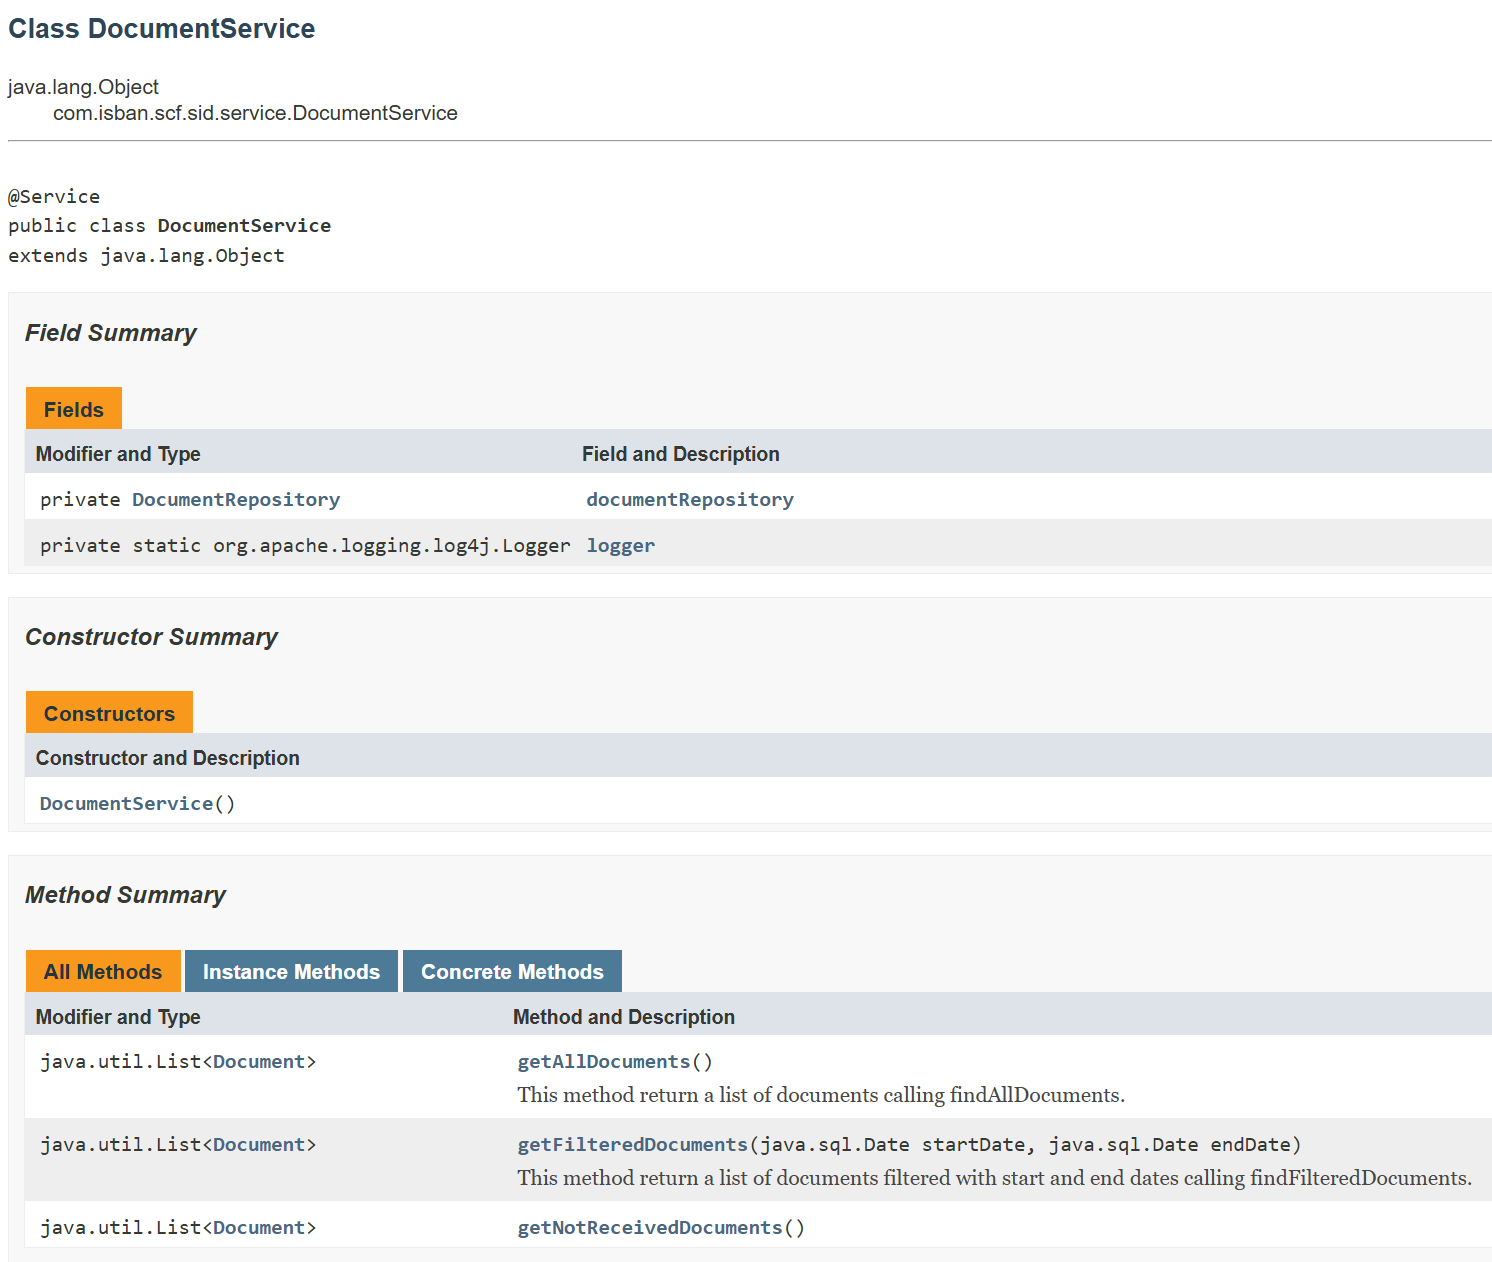
\includegraphics[width=0.5\linewidth]{javadoc-SIDManager.png}
%     \caption{Interfaz web de Javadoc para la clase \emph{DocumentService}}
%     \label{fig:javadoc-document-service}
% \end{figure}


% La implementación de Javadoc en la aplicación no solo mejora la comprensión del código para los desarrolladores, sino que también facilita su uso y mantenimiento. Esta práctica sigue los estándares de la industria y garantiza que cualquier persona que desee utilizar o modificar la aplicación pueda hacerlo de manera eficiente y con un mínimo de esfuerzo.



